% Title page
\frame[plain]{\titlepage}

\lecture{Введение}{intro}

\section{Факты, правила и запросы}
\subsection{Основные пункты}

\begin{frame}
	\frametitle{\insertsection}
	\framesubtitle{\insertsubsection}
	\begin{itemize}
		\item Рассмотреть простые примеры программ на \textbf{Prolog}, определить понятия факта, правила, запроса и базы знаний
		\item Дать определения основных понятий и синтаксических конструкций, таких как атомы, переменные и термы
	\end{itemize}
\end{frame}

\subsection{База знаний}

\begin{frame}
	\frametitle{\insertsection}
	\framesubtitle{\insertsubsection}
	Базовые конструкции языка \textbf{Prolog}:
	\begin{itemize}
		\item Факты
		\item Правила
		\item Запросы
	\end{itemize}
	Программа на Prolog представляет собой множество \textbf{фактов} и \textbf{правил}~--- \alert{Базу Знаний}
	Чтобы использовать информацию, содержащуюся в базе знаний, необходимо ставить \textbf{запросы}.
\end{frame}

\begin{frame}
	\frametitle{\insertsection}
	\framesubtitle{\insertsubsection}
	Пример 1
	
	
	\texttt{\begin{itemize}
				\item[] woman(mia).
				\item[] woman(jody).
				\item[] woman(yolanda).
				\item[] playsGuitar(jody).
				\item[]<2-> listensToMusic(mia).
				\item[]<2-> musician(yolanda).
				\item[]<2-> playsGuitar(mia) :- listensToMusic(mia).
				\item[]<2-> playsGuitar(yolanda) :- listensToMusic(yolanda).
				\item[]<2-> listensToMusic(yolanda) :- musician(yolanda).
			\end{itemize}}
\end{frame}

\begin{frame}
	\frametitle{\insertsection}
	\framesubtitle{\insertsubsection}
	Пример 2
	
	
	\texttt{\begin{itemize}
		\item[] musician(mia).
		\item[] listensToMusic(jody).
		\item[] playsGuitar(mia) :- listensToMusic(mia),musician(mia).
		\item[] playsGuitar(jody) :- musician(jody); listensToMusic(jody).
	\end{itemize}}
\end{frame}

\begin{frame}
	\frametitle{\insertsection}
	\framesubtitle{\insertsubsection}
	Пример 3
	
	
	\texttt{\begin{itemize}
		\item[] woman(mia).
		\item[] woman(jody).
		\item[] woman(yolanda).
		\item[] loves(vincent,mia).
		\item[] loves(marcellus,mia).
	\end{itemize}}
\end{frame}

\begin{frame}
	\frametitle{\insertsection}
	\framesubtitle{\insertsubsection}
	Пример 4
	
	
	\texttt{\begin{itemize}
			\item[] loves(vincent,mia).
			\item[] loves(marcellus,mia).
			\item[] jealous(X,Y) :- loves(X,Z),loves(Y,Z).
	\end{itemize}}
\end{frame}

\subsection{Синтаксис}

\begin{frame}
	\frametitle{\insertsection}
	\framesubtitle{\insertsubsection}
	\textbf{\underline{Атомы}}
	
	\begin{enumerate}
		\item Последовательность строчных или прописных букв, цифр и символов подчерка, начинающаяся со строчной буквы.
		\item Произвольная последовательность символов, заключённая в одинарные кавычки.
		\item Последовательность спецсимволов.
	\end{enumerate}

	\begin{rexample}
		mia, marcellus, big\_kahuna\_burger, 'Произвольная строка символов', ====>, :-
	\end{rexample}
\end{frame}

\begin{frame}
	\frametitle{\insertsection}
	\framesubtitle{\insertsubsection}
	\textbf{\underline{Числа}}
	
	\begin{enumerate}
		\item Действительные числа: 2,718; 103,3087; \(\pi \), \ldots
		\item Целые числа: -2, -1, 0, 1, 2, \ldots
	\end{enumerate}

	\textbf{\underline{Переменные}}
	
	
	\textbf{Переменные} служат для обозначения объектов, значения которых меняются в ходе выполнения программы. Имя переменной задается
	последовательностью строчных или прописных букв, цифр и символов подчерка, начинающейся с \textbf{прописной буквы} или \textbf{символа подчерка}.
	
	\begin{rexample}
		X, Y, Variable, \_X, X1, \_variable\_with\_some\_info\_
	\end{rexample}
\end{frame}

\begin{frame}
	\frametitle{\insertsection}
	\framesubtitle{\insertsubsection}
	\textbf{\underline{Термы}}
	
	\textit{Терм (составной терм)} состоит из \alert{функтора} и последовательности аргументов в скобках.
	\begin{enumerate}
		\item Любой атом или число является термом. Такие термы называются \alert{константами}.
		\item Любая переменная является термом.
		\item Имя функтора~--- это атом.
		\item Переменная не может быть функтором.
		\item Аргументы составного терма должны быть термами.
	\end{enumerate}

	\begin{rexample}
		loves(vincent, mia), playsGuitar(jody), jody, musician(mia), eats(cat,Prey)
	\end{rexample}
\end{frame}

\subsection{Проверочные вопросы}

\begin{frame}
	\frametitle{\insertsection}
	\framesubtitle{\insertsubsection}
	Какие из перечисленных строк являются атомами, какие переменными, а какие не являются ни тем, ни другим?
	\texttt{\begin{enumerate}
		\item vINCENT
		\item Foot
		\item x1
		\item Y3
		\item big\_kahuna\_burger
		\item 'Криминальное чтиво'
		\item roast chicken
		\item \_IndianaJones
		\item '\_IndianaJones'
	\end{enumerate}}
\end{frame}

\begin{frame}
	\frametitle{\insertsection}
	\framesubtitle{\insertsubsection}
	Какие из перечисленных ниже строк являются атомами, переменными или составными термами, а какие вообще не являются термами? Для каждого составного терма укажите имя функтора и его арность.
	\texttt{\begin{enumerate}
		\item loves(vincent,mia)
		\item 'loves(vincent,mia)'
		\item Eats(cat,mouse)
		\item hasChildren(cat,kittens)
		\item and(musician(jody),artist(mia))
		\item and(musician(X),artist(Y))
		\item \_and(musician(jody),artist(mia))
		\item (Butch kills Vincent)
		\item kills(Butch,Vincent)
		\item kills(Butch,Vincent
	\end{enumerate}}
\end{frame}

\begin{frame}
	\frametitle{\insertsection}
	\framesubtitle{\insertsubsection}
	Сколько фактов, правил, высказываний и предикатов в следующей базе знаний? Для каждого правила назовите вывод и цели.
	\texttt{\begin{itemize}
			\item[] woman(mia).
			\item[] woman(jody).
			\item[] man(jules).
			\item[] person(X) :- man(X); woman(X).
			\item[] loves(X,Y) :- knows(Y,X).
			\item[] father(Y,Z) :- man(Y), son(Z,Y).
			\item[] father(Y,Z) :- man(Y), daughter(Z,Y).
	\end{itemize}}
\end{frame}

\subsection{Упражнения}

\begin{frame}
	\frametitle{\insertsection}
	\framesubtitle{\insertsubsection}
	Запишите следующую базу знаний на языке Prolog.
	
	\begin{itemize}
		\item Бутч убийца.
		\item Миа и Марселлас женаты.
		\item Зед мертв.
		\item Марселлас убьет любого, кто сделает Мие массаж стопы.
		\item Миа любит любого, кто хорошо танцует.
		\item Джулс ест все, что вкусно или питательно.
	\end{itemize}
\end{frame}

\begin{frame}
	\frametitle{\insertsection}
	\framesubtitle{\insertsubsection}
	Пусть дана следующая база знаний:
	\texttt{\begin{itemize}
			\item[] sportsman(john).
			\item[] hasUniform(harry).
			\item[] footballPlayer(harry).
			\item[] sportsman(X) :- isTrained(X),hasUniform(X).
			\item[] isTrained(X) :- footballPlayer(X).
	\end{itemize}}
	
	Как Prolog ответит на следующие запросы?
	\texttt{\begin{enumerate}
			\item sportsman(john).
			\item footballPlayer(john).
			\item sportsman(harry).
			\item sportsman(X).
			\item hockeyPlayer(john).
	\end{enumerate}}
\end{frame}

\subsection{Дополнительное задание}

\begin{frame}
	\frametitle{\insertsection}
	\framesubtitle{\insertsubsection}
	Средствами языка Prolog \textbf{определить, какие животные не имеют хозяина.}
	\begin{enumerate}
		\item Бутси~--- коричневая кошка.
		\item Корни~--- черная кошка.
		\item Мак~--- рыжая кошка.
		\item Флэш, Ровер и Спот~--- собаки, Ровер~--- рыжая, а Спот~--- белая.
		\item Все животные, которыми владеют Том и Кейт, имеют родословные.
		\item Том владеет всеми черными и коричневыми животными, а Кейт владеет всеми собаками небелого цвета, которые не являются собственностью Тома.
		\item Алан владеет Мак, если Кейт не владеет Бутси и если Спот не имеет родословной.
		\item Флэш~--- пятнистая собака.
	\end{enumerate}
\end{frame}

\lecture{Matching}{match}

\section{Унификация термов и поиск решений}
\subsection{Основные пункты}

\begin{frame}
	\frametitle{\insertsection}
	\framesubtitle{\insertsubsection}
	\begin{itemize}
		\item Познакомиться с понятием согласования термов.
		\item Разобраться в стратегиях, используемых интерпретатором языка Prolog для поиска ответов на вопросы.
	\end{itemize}
\end{frame}

\subsection{Определение}

\begin{frame}
	\frametitle{\insertsection}
	\framesubtitle{\insertsubsection}
	\only<1>{Два терма \alert{унифицированы}, если они равны или если они содержат переменные и существует означивание этих переменных, такое, что термы становятся равными.}
	\only<2->{\begin{enumerate}
			\item Если \texttt{term1} и \texttt{term2} константы, то \texttt{term1} и \texttt{term2} унифицированы тогда и только тогда, когда они равны друг другу, т.е. \texttt{term1} и \texttt{term2} это один и тот же атом или число.
			\item Если \texttt{term1}~--- это переменная, а \texttt{term2}~--- любой терм, то термы \texttt{term1} и \texttt{term2} унифицированы, и переменная \texttt{term1} инициализируется значением терма \texttt{term2}. 
			Если \texttt{term1} и \texttt{term2}~--- переменные, они унифицированы и принимают значения друг друга. Говорят, что переменные \texttt{term1} и \texttt{term2} \alert{разделяют значение}.
			\item Если \texttt{term1} и \texttt{term2} составные термы, то они унифицированы тогда и только тогда, когда:
			\begin{enumerate}[(a)]
				\item Их функторы и арность совпадают.
				\item Соответствующие аргументы обоих термов унифицированы. При этом означивание переменных согласовано.
			\end{enumerate}
			\item Два терма унифицированы тогда и только тогда, когда это следует из одного из предыдущих пунктов.
	\end{enumerate}}
\end{frame}

\subsection{Примеры унификации}

\begin{frame}
	\frametitle{\insertsection}
	\framesubtitle{\insertsubsection}
	\textbf{Какие из термов унифицированы?}
	\texttt{\begin{itemize}
		\item john = john.
		\item 42 = 42.
		\item 'Строка слов' = 'Строка слов'.
		\item 'mia' = mia.
		\item '42' = 42.
		\item mia = X.
		\item X = Y.
		\item kill(shoot(gun),Y) = kill(X,stab(knife)).
		\item loves(X,X) = loves(marcellus,mia).
		\item parent(A) = A.
	\end{itemize}}
\end{frame}

\subsection{Поиск решений}

\begin{frame}
	\frametitle{\insertsection}
	\framesubtitle{\insertsubsection}
	Интерпретатор языка Prolog обрабатывает условия запроса последовательно слева направо. Для каждого из условий интерпретатор ищет унифицируемый с ним факт или вывод правила, проходя базу знаний сверху вниз.
\end{frame}

\begin{frame}
	\frametitle{\insertsection}
	\framesubtitle{\insertsubsection}
	\texttt{\begin{itemize}
			\item[] person(vincent).
			\item[] person(jules).
			\item[] hasGun(vincent).
			\item[] hasGun(jules).
			\item[] alive(jules).
			\item[] lucky(X) :- person(X),hasGun(X),alive(X).
	\end{itemize}}
\end{frame}

\subsection{Дерево поиска решений}

\begin{frame}
	\frametitle{\insertsection}
	\framesubtitle{\insertsubsection}
	\begin{figure}
		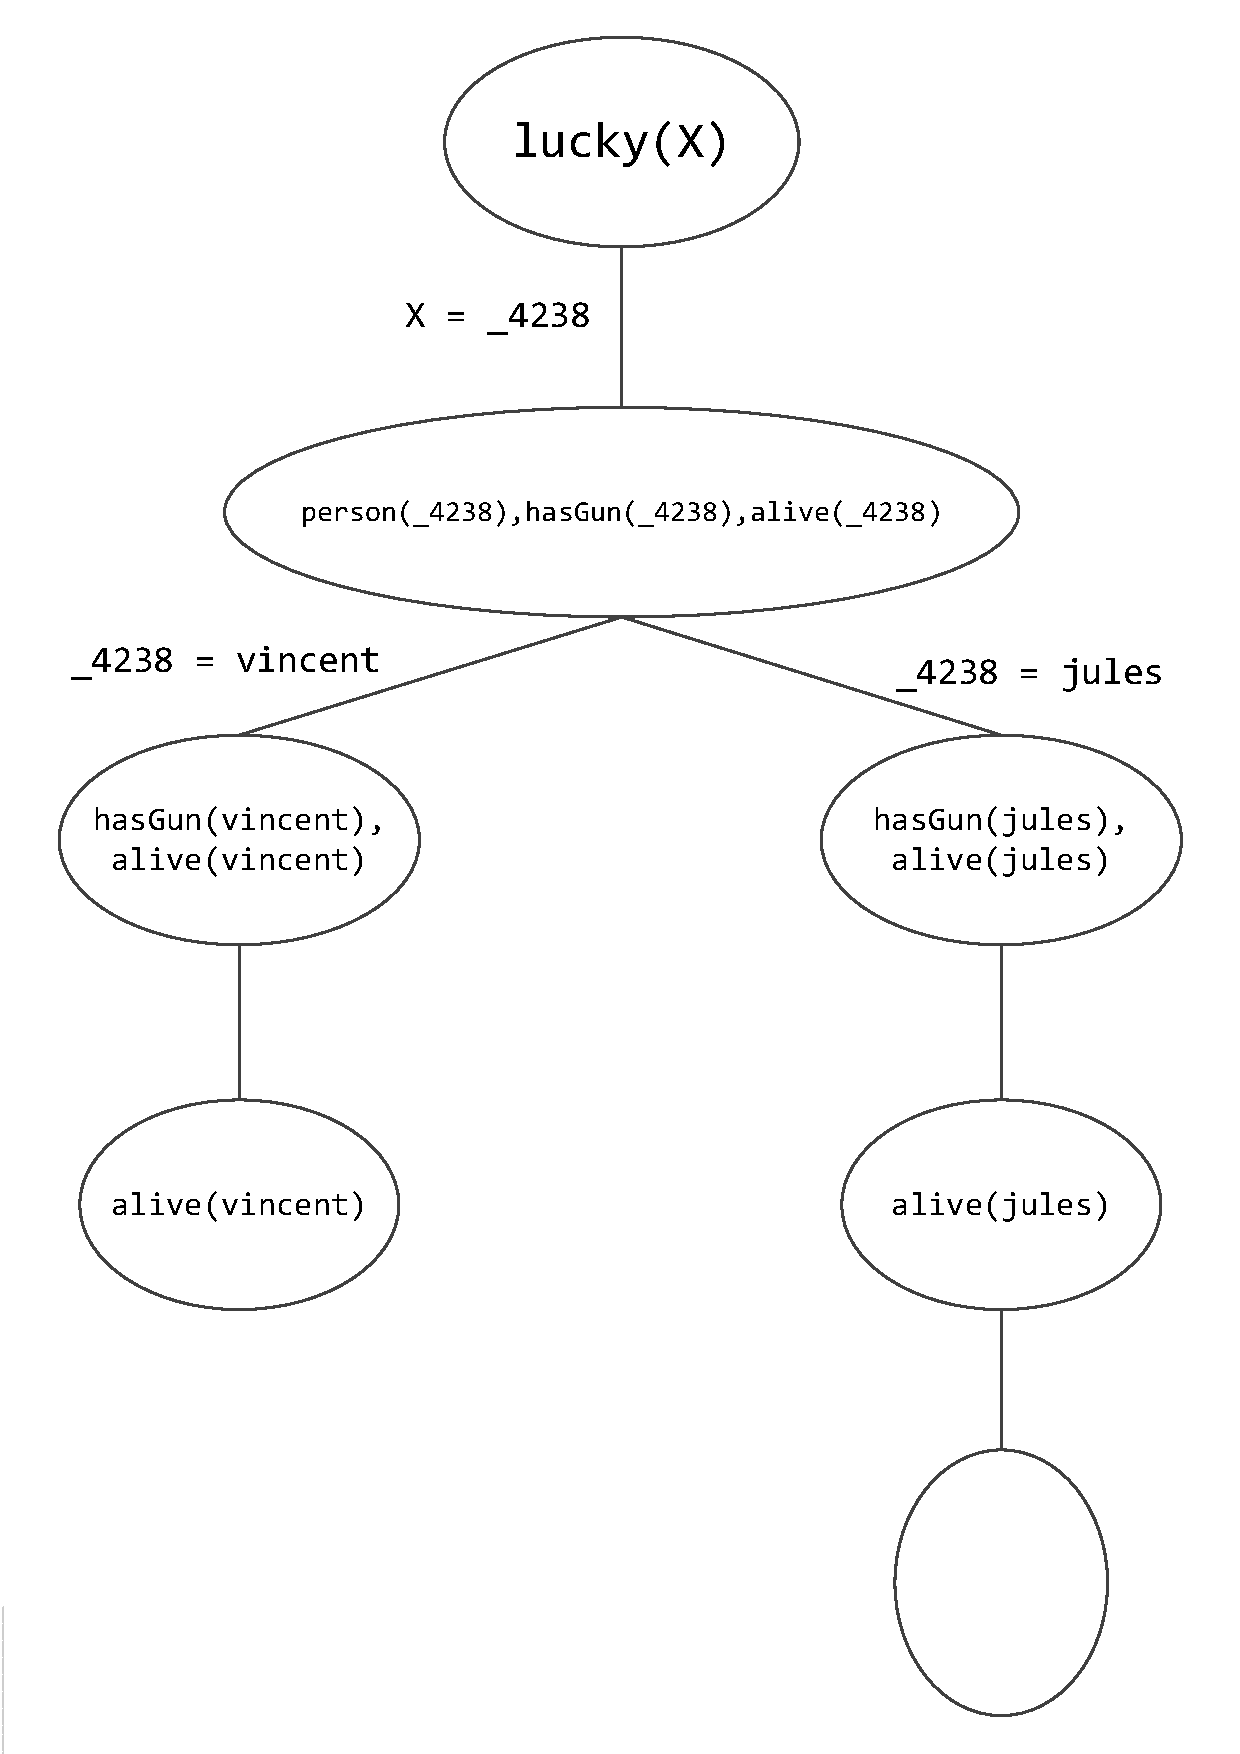
\includegraphics[scale=0.35]{stree}
	\end{figure}
\end{frame}

\subsection{Упражнения}

\begin{frame}
	\frametitle{\insertsection}
	\framesubtitle{\insertsubsection}
	В каких из перечисленных пар термы унифицированы? Где необходимо запишите значения переменных, необходимые для унификации.
	\texttt{\begin{enumerate}
			\item bread = bread.
			\item 'Bread' = bread.
			\item 'bread' = bread.
			\item Bread = bread.
			\item хлеб = котлета.
			\item food(bread) = bread.
			\item food(bread) = Bread.
			\item food(Bread) = food(bread).
			\item food(хлеб,X) = food(Y,котлета).
			\item graph(edge(v1,v2),X,edge(Y,v4)) = graph(Z,edge(v7,v8),edge(v4,X)).
			\item food(X) = X.
			\item meal(food(bread),drink(beer)) = meal(food(X),Y).
			\item meal(food(bread),X) = meal(X,drink(beer)).
	\end{enumerate}}
\end{frame}

\begin{frame}
	\frametitle{\insertsection}
	\framesubtitle{\insertsubsection}
	\textbf{Пусть дана следующая база знаний.}
	\texttt{\begin{itemize}
			\item[] witch(gullveig).
			\item[] god(freyja).
			\item[] god(odin).
			\item[] god('Vidarr').
			\item[] magic(X) :- witch(X).
			\item[] magic(X) :- wizard(X).
			\item[] magic(X) :- god(X).
	\end{itemize}}
	\textbf{Каким из запросов она удовлетворяет?}
	\texttt{\begin{enumerate}
			\item magic(witch).
			\item wizard(odin).
			\item magic('Vidarr').
			\item magic(Vidarr).
	\end{enumerate}}
\end{frame}

\begin{frame}
	\frametitle{\insertsection}
	\framesubtitle{\insertsubsection}
	\textbf{Дан следующий лексикон.}
	\texttt{\begin{itemize}
			\item[] word(article,a).
			\item[] word(article,every).
			\item[] word(noun,criminal).
			\item[] word(noun,'big kahuna burger').
			\item[] word(verb,eats).
			\item[] word(verb,likes).
%			\item[] sentence(W1,W2,W3,W4,W5) :- word(article,W1), word(noun,W2), word(verb,W3), word(article,W4), word(noun,W5).
	\end{itemize}}
	Написать запрос на получение списка всех возможных фраз данного лексикона, имеющих вид: \textit{артикль+существительное+глагол+артикль+существительное}. Построить дерево поиска решений для одной из построенных фраз.
\end{frame}

\begin{frame}
	\frametitle{\insertsection}
	\framesubtitle{\insertsubsection}
	Имеется следующий список слов: \textit{бок, акр, сомо, бокс, хата, эдда, вино, рода, окот, анод, скала, онагр, обиход, монако, дверка, дигора, удокан, маарри, бинокль, бегония}.
	Пусть в базе знаний слова представляются следующим образом:
	\texttt{\begin{itemize}
			\item[] word(эдда,э,д,д,а).
			\item[] word(вино,в,и,н,о).
			\item[] word(рода,р,о,д,а).
			\item[] word(окот,о,к,о,т).
			\item[] word(анод,а,н,о,д).
			\item[] word(скала,с,к,а,л,а).
			\item[] word(онагр,о,н,а,г,р).
			\item[] word(обиход,о,б,и,х,о,д).
	\end{itemize}}
\end{frame}

\begin{frame}
	\frametitle{\insertsection}
	\framesubtitle{\insertsubsection}
	Реализовать предикат \texttt{crosswd/10 = crosswd(V1,V2,V3,V4,V5,V6,H1,H2,H3,H4)}, который бы заполнял данными словами следующий кроссворд таким образом, чтобы
	слова, идущие вертикально, были первыми 6 аргументами, а слова, идущие горизонтально~--- последними.
	\begin{figure}
		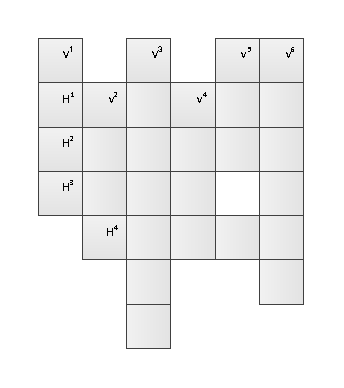
\includegraphics[scale=0.9]{crosswd}
	\end{figure}
\end{frame}

\lecture{Recursion}{recursion}

\begin{frame}[plain,c]

	\begin{center}
		\Huge Определения и примеры
	\end{center}

\end{frame}

\section{Рекурсия в Prolog}
\subsection{Простой пример}

\begin{frame}
	\frametitle{\insertsection}
	\framesubtitle{\insertsubsection}
	\texttt{\begin{itemize}
			\item[] переваривает(Хищник,Добыча) :- съел(Хищник,Добыча).
			\item[] переваривает(Хищник,Добыча) :- съел(Хищник,ДругойХищник), переваривает(ДругойХищник,Добыча).
			\item[] съел(комар,кровь).
			\item[] съел(лягушка, комар).
			\item[] съел(цапля, лягушка).
	\end{itemize}}
\end{frame}

\section{Уровни понимания программ}
\subsection{Декларативный и процедурный}

\begin{frame}
	\frametitle{\insertsection}
	\framesubtitle{\insertsubsection}
	\alert{Декларативный смысл} Prolog-программы касается только \textit{отношений}, определенных в программе.
	Другими словами, декларативный смысл определяет, что должно быть результатом работы программы с точки зрения математической логики.
	
	\alert{Процедурный смысл} программы определяет еще и как этот результат был получен, т.е. как отношения реально обрабатываются пролог-системой.
\end{frame}

\section{Правила описания рекурсивных предикатов}
\subsection{База и шаг рекурсии}

\begin{frame}
	\frametitle{\insertsection}
	\framesubtitle{\insertsubsection}
	\only<1>{\textbf{База рекурсии}}
	\only<2>{\textbf{Шаг рекурсии}}
	
	
	\texttt{\begin{itemize}
			\item[] {\color<1>[RGB]{0,0,255}{переваривает(Хищник,Добыча) :- съел(Хищник,Добыча).}}
			\item[] {\color<2>[RGB]{0,0,255}{переваривает(Хищник,Добыча) :- съел(Хищник,ДругойХищник), переваривает(ДругойХищник,Добыча).}}
			\item[] съел(комар,кровь).
			\item[] съел(лягушка, комар).
			\item[] съел(цапля, лягушка).
	\end{itemize}}
\end{frame}

\subsection{descending.pl}

\begin{frame}
	\frametitle{\insertsection}
	\framesubtitle{\insertsubsection}
	\texttt{\begin{itemize}
			\item[] child(adam,cain).
			\item[] child(adam,abel).
			\item[] child(adam,seth).
			\item[] child(cain,enoch).
			\item[] child(enoch,irad).
			\item[] child(irad,mehujael).
			\item[] child(seth,enos).
			\item[] child(enos,kenan).
			\item[] child(kenan,mahalalel).
			\item<2->[] descend(A,D) :- child(A,D).
			\item<2->[] descend(A,D) :- child(A,C), descend(C,D).
	\end{itemize}}
\end{frame}

\subsection{arithmetic.pl}

\begin{frame}
	\frametitle{\insertsection}
	\framesubtitle{\insertsubsection}
	\texttt{\begin{itemize}
			\item[] num(0).
			\item[] num(s(N)) :- num(N).
			\item<2->[] plus(0,N,N).
			\item<2->[] plus(s(M),N,s(Sum)) :- plus(M,N,Sum).
	\end{itemize}}
\end{frame}

\section{Рекурсия и хвостовая рекурсия}
\subsection{Численная арифметика: вычисление факториала числа}

\begin{frame}
	\frametitle{\insertsection}
	\framesubtitle{\insertsubsection}
	
	\texttt{\begin{itemize}
			\item[] f(0,1).
			\item[] f(X,Y) :- X>0,X1 is X-1,f(X1,Y1),Y is Y1*X.
	\end{itemize}}

	\uncover<2->{\texttt{\begin{itemize}
				\item[] f(N,N,F):-write(F),!.
				\item[] f(N,N1,F1):- N2 is N1+1,F2 is F1*N2,f(N,N2,F2).
				\item[] factorial(N):- f(N,1,1).
	\end{itemize}}}

\end{frame}

\section{Последовательность целей и остановка программ}
\subsection{Возможные источники ошибок}

\begin{frame}

	\frametitle{\insertsection}
	\framesubtitle{\insertsubsection}
	\texttt{\begin{itemize}
			\item[] child(adam,cain).
			\item[] child(adam,abel).
			\item[] child(adam,seth).
			\item[] child(cain,enoch).
			\item[] child(enoch,irad).
			\item[] child(irad,mehujael).
			\item[] child(seth,enos).
			\item[] child(enos,kenan).
			\item[] child(kenan,mahalalel).
	\end{itemize}}
	\texttt{\only<1>{\begin{itemize}
				\item[] descend(A,D) :- child(A,D).
				\item[] descend(A,D) :- child(A,C), descend(C,D).
			\end{itemize}}
		\only<2>{\begin{itemize}
				\item[] descend(A,D) :- descend(C,D), child(A,C).
				\item[] descend(A,D) :- child(A,D).
		\end{itemize}}
		\only<3>{\begin{itemize}
				\item[] descend(A,D) :- child(A,D).
				\item[] descend(A,D) :- descend(C,D), child(A,C).
		\end{itemize}}
		\only<4>{\begin{itemize}
				\item[] descend(A,D) :- child(A,C), descend(C,D).
				\item[] descend(A,D) :- child(A,D).
		\end{itemize}}
	}

\end{frame}

\begin{frame}

	\frametitle{\insertsection}
	\framesubtitle{\insertsubsection}
	
	\texttt{\begin{itemize}
			\item[] num(0).
			\item[] num(s(N)) :- num(N).
		\end{itemize}
	}
	
	\texttt{\begin{itemize}
			\item[] num(s(N)) :- num(N).
			\item[] num(0).
		\end{itemize}
	}

\end{frame}

\begin{frame}[plain,c]

	\begin{center}
		\Huge Упражнения
	\end{center}

\end{frame}


\section{Упражнения}

\begin{frame}
	\frametitle{\insertsection}
	\begin{itemize}
		\item Скачайте или перепишите листинг программы \texttt{descending.pl}. Рассмотрите каждый случай рекурсии (см. слайды ранее). Какие запросы работают, какие нет? Почему?
		\item Скачайте или перепишите листинг программы \texttt{arithmetic.pl}. Реализуйте следующие операции над числами, определенными в программе:
		\begin{enumerate}
			\item \textbf{Умножение}: реализуйте предикат \texttt{times/3}, такой, чтобы последним аргументом было произведение двух первых.
			\item \textbf{Возведение в степень}: реализуйте предикат \texttt{exp(N,X,R)}, такой, чтобы \(R = X^{N}\).
			\item \textbf{Сравнение}: реализуйте предикаты \texttt{gt/2, lt/2}, истинные тогда, когда первый аргумент больше (меньше), чем второй.
			\item \textbf{Равенство}: реализуйте предикат \texttt{eq/2}, истинный тогда и только тогда, когда его аргументы равны.
			\item \textbf{Максимум и минимум двух чисел}: реализуйте предикаты \texttt{max/3, min/3}, где третий аргумент~--- это максимум (минимум) из двух первых.
		\end{enumerate}
	\end{itemize}
\end{frame}

\begin{frame}
	\frametitle{\insertsection}
	\begin{itemize}
		\item Реализуйте программу для вычисления факториала числа (в обычной численной арифметике). Сравните время работы и количество операций в зависимости от значения входных параметров.
		\item Реализуйте программу для вычисления чисел Фибоначчи. Реализуйте предикат \texttt{getFibN/2 = getFibN(N, Fn)}, такой, что \(F_n\)~--- N-е число Фибоначчи.
		\item Используя предыдущую программу, реализуйте предикат \texttt{getNearestFibonacci/3}, возвращающий по заданному числу номер ближайшего к нему числа Фибоначчи и его номер.
	\end{itemize}
\end{frame}



\lecture{Additional Excercises}{recursionExt}

\section{Дополнительные упражнения}

\begin{frame}
	
	\frametitle{\insertsection}
	
	Преобразуйте программу \texttt{arithmetic.pl}.
	
	\begin{itemize}
		\item Реализуйте операцию деления \(N\) на \(M\) с остатком таким образом, чтобы результатом были два числа \(Q\) и \(P\), такие, что \(N = M\cdot Q + P \).
		\item Реализуйте алгоритм Евклида для поиска наибольшего общего делителя двух заданных чисел.
	\end{itemize}
	
\end{frame}

\begin{frame}
	\frametitle{\insertsection}
	Опишите следующий граф в виде базы знаний. Реализуйте предикат \texttt{fromTo/2 = fromTo(Begin,End)}, который по заданным началу и концу маршрута будет выяснять, существует ли путь между
	заданными вершинами и печатать в консоли слово, которое получается при следовании по найденному пути.
	
	\begin{figure}
		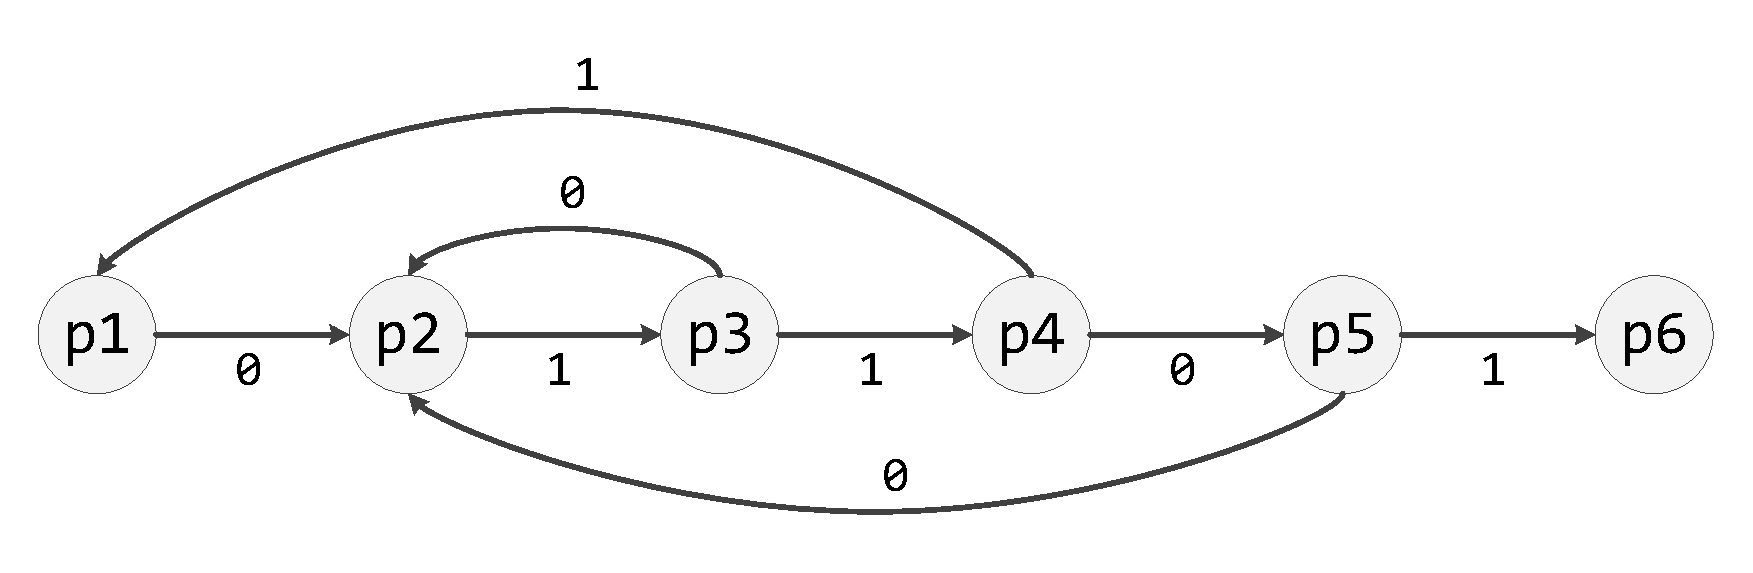
\includegraphics[scale=0.35]{graph}
	\end{figure}
\end{frame}

\begin{frame}[shrink=7]
	\frametitle{\insertsection}
	Скачайте базу знаний \texttt{travel.pl} или перепишите.
	\texttt{\begin{itemize}
		\item[] byCar(auckland,hamilton).
		\item[] byCar(hamilton,raglan).
		\item[] byCar(valmont,saarbruecken).
		\item[] byCar(valmont,metz).
		\item[] byTrain(metz,frankfurt).
		\item[] byTrain(saarbruecken,frankfurt).
		\item[] byTrain(metz,paris).
		\item[] byTrain(saarbruecken,paris).
		\item[] byPlane(frankfurt,bangkok).
		\item[] byPlane(frankfurt,singapore).
		\item[] byPlane(paris,losAngeles).
		\item[] byPlane(bangkok,auckland).
		\item[] byPlane(losAngeles,auckland).
	\end{itemize}}
	Реализуйте предикат \texttt{travel/2}, который по заданным началу и концу маршрута определял бы, существует ли способ добраться из начала в конец и
	печатал пункты маршрута, а также виды транспорта, которыми осуществляется перемещение между промежуточными пунктами.
\end{frame}

\begin{frame}[plain,c]

\begin{center}
	\Huge Домашнее задание
\end{center}

\end{frame}

\section{Домашнее задание}

\begin{frame}
	
	\frametitle{\insertsection}
	
	
	Реализуйте некоторый каталог вида \texttt{unit(key, value)}. Например, список книг по авторам:
	\texttt{\begin{itemize}
			\item[] book(heinlein, 'Stranger in a Strange Land').
			\item[] book(heinlein, 'The Moon Is a Harsh Mistress').
			\item[] book(niven, 'Lucifer's Hammer').
	\end{itemize}}
	
	Реализуйте программу, запрашивающую из консоли ввод автора и печатающую либо список его книг, либо сообщение, что книг данного автора в каталоге нет.
	
	
	\alert{Также на дом остается реализация программы travel.pl с предыдущего слайда, если это не было сделано на занятиях.}
	
\end{frame}


% Списки в Prolog


\lecture{Lists}{lists}

\begin{frame}[plain,c]

	\begin{center}
		\Huge Понятие и вид списка в Prolog
	\end{center}

\end{frame}

\section{Списки}

\subsection{Список в Prolog}

\begin{frame}
	\frametitle{\insertsection}
	\framesubtitle{\insertsubsection}
	
	\begin{itemize}
		\item Списком называют конечную последовательность элементов.
		\item В синтаксисе языка Prolog границы списка определяются квадратными скобками [ и ].
		\item Элементы списка отделяются друг от друга запятой. Элементами списка могут быть любые термы.
		\item Любой непустой список можно разделить на голову и хвост (head и tail). Для записи используется специальный символ |. 
		\texttt{[Head | Tail] = [one, two, three]} => \texttt{Head = one, Tail = [two, three]}. Голова списка~--- это элемент,
		хвост списка~--- это список.
		\item Пустой список не может быть разделен на голову и хвост.
	\end{itemize}

\end{frame}

\subsection{Простой пример}

\begin{frame}

	\frametitle{\insertsection}
	\framesubtitle{\insertsubsection}
	
	\texttt{\begin{itemize}
			\item[] []
			\item[] [first, second, third, fourth, fifth]
			\item[] [1, 2, 3, 4, 5, 6, 7, 8, 9, 0]
			\item[] [first, 2, color(cornie, black), F, fifth, F]
			\item[] [first, second, [third, fourth], [fifth, color(cornie, black)]]
			\item[] [[], [], car(volkswagen), F, 1, 2, [1, F, car(bmw), [1, 2, 4]], X]
	\end{itemize}}

\end{frame}

\subsection{Получение элементов списка}

\begin{frame}

	\frametitle{\insertsection}
	\framesubtitle{\insertsubsection}
	
	\texttt{\begin{itemize}
			\item[] [abyssian, bobtail, [bengal, birman]]
	\end{itemize}}

	\texttt{\begin{itemize}
			\item<2-> {[H|T]} = [abyssian, bobtail, [bengal, birman]].
			\item<3-> {[F,S|T]} = [abyssian, bobtail, [bengal, birman]].
			\item<4-> {[\_,S|T]} = [abyssian, bobtail, [bengal, birman]].
			\item<5-> {[First,\_,\_,Fourth|\_]} = [abyssian, bobtail, [bengal, birman]].
			\item<6-> {[\_,\_,[\_|T]|\_]} = [abyssian, bobtail, [bengal, birman]].
	\end{itemize}}

\end{frame}

\section{Операции со списками}
\subsection{Проверка вхождения элемента}

\begin{frame}
	
	\frametitle{\insertsection}
	\framesubtitle{\insertsubsection}
	
	Предикат \alert{\texttt{member/2 = member(?Elem, ?List)}} имеет два аргумента~--- некоторый терм и список, и принимает значение \texttt{true} в
	случае, когда \texttt{?Elem} содержится в списке \texttt{?List}. В противном случае предикат принимает значение \texttt{false}.
	\newline \newline
	\uncover<2->{Как можно реализовать предикат \texttt{member/2} самостоятельно?}
	
	\texttt{\begin{itemize}
			\item<3->[] member(X, [X|T]).
			\item<4->[] member(X, [H|T]) :- member(X,T).
	\end{itemize}}

	\uncover<5->{\texttt{\begin{itemize}
				\item[] member(X, [X|\_]).
				\item[] member(X, [\_|T]) :- member(X,T).
	\end{itemize}}}
	
\end{frame}

\subsection{Другие операции}

\begin{frame}

	\frametitle{\insertsection}
	\framesubtitle{\insertsubsection}
	
	\begin{itemize}
		\item Подсчет длины списка.
		\item Конкатенация двух списков.
		\item Поиск префикса, суффикса и подсписка заданного списка.
		\item Поиск последнего элемента списка.
		\item Обращение списка
		\item Сортировка.
	\end{itemize}

\end{frame}


\begin{frame}[plain,c]
	
	\begin{center}
		\Huge Домашнее задание
	\end{center}

\end{frame}

\section{Домашнее задание}

\begin{frame}
	
	\frametitle{\insertsection}
	
	\begin{enumerate}
		\item В программе \texttt{lists.pl} реализовать предикат \texttt{revAcc}, обращающий список более эффективно, чем
		предикат \texttt{rev}. Использовать дополнительный список для аккумуляции результата.
		\item В программу \texttt{lists.pl} добавить реализацию предиката \texttt{listGen}, генерирующего по заданному числу N
		список длины N, заполненный случайными целыми числами (см. предикаты \texttt{randon} и \texttt{random\_between}).
		\item Реализовать в программе \texttt{lists.pl} алгоритм быстрой сортировки quicksort двумя способами и сравните их
		производительность на списках большой длины. Для разделения списка можно использовать встроенный предикат \texttt{partition/4}.
		\begin{enumerate}
			\item Реализовать предикат \texttt{qsortLast}, который в качестве опорного берет последний элемент списка.
			\item Реализовать предикат \texttt{qsortMiddle}, где в качестве опорного берется центральный элемент списка.
		\end{enumerate}
		\item Изменить программу \texttt{monkey.pl} так, чтобы избежать генерации бесконечного множества
		абстрактных решений.
	\end{enumerate}
	
\end{frame}


% Арифметика и численные операции


\lecture{Arithmetic}{arithmetic}


\begin{frame}
	
	\begin{center}
		\Huge Арифметика в Prolog
	\end{center}
	
\end{frame}


\section{Реализация арифметики в Prolog}
\subsection{Численные типы и операции}

\begin{frame}

	\frametitle{\insertsection}
	\framesubtitle{\insertsubsection}
	
	В языке Prolog реализованы численные типы данных и операции над ними.
	Для проверки типов в программе применяются соответствующие встроенные предикаты.
	
	Численные типы данных:
	
	\begin{itemize}
		\item \textbf{Integer} --- целые числа: \(1, 2, 3, 4, -100, 1001 \). Предикат \texttt{integer/1} возвращает \texttt{True} в случае, если переданный терм представляет целое число.
		\item \textbf{Float} --- вещественные числа: \(1.2, 3.14, 2.7 \). Предикат \texttt{float/1} возвращает \texttt{True}, если терм представляет вещественное число.
		\item \textbf{Rational} --- рациональные числа: \(\frac{1}{3}, \frac{2}{7} \). Для проверки используется предикат \texttt{rational/1}. Данный предикат считает рациональными и все целые числа.
	\end{itemize}

	Рациональные числа записываются с помощью специального предиката \texttt{rdiv}, который работает как дробная черта.
	
	\begin{rexample}
		\(\frac{1}{3}  = \) \texttt{1 rdiv 3}.
		\texttt{X is (1 rdiv 3) * 3 \( \Rightarrow \) X = 1.}
	\end{rexample}

\end{frame}


\begin{frame}
		
		\frametitle{\insertsection}
		\framesubtitle{\insertsubsection}
		
		\begin{table}
			\centering
			\begin{tabular}{ l | r }
				\rowcolor{Gray}
				\textbf{Арифметическое выражение} & \textbf{Запись в синтаксисе Prolog} \\
				\hline
				\rowcolor{LightGray}\( 10 + 5 = 15 \) & \texttt{15 is 10 + 5.}   \\
				\rowcolor{LightGray}\( 10\cdot 5 = 50 \)  & \texttt{50 is 10 * 5.}   \\
				\rowcolor{LightGray}\( 10 - 5 = 5 \)  & \texttt{5 is 10 - 5.}   \\
				\rowcolor{LightGray}\( 5 - 10 = -5 \)  & \texttt{-5 is 5 - 10.}   \\
				\rowcolor{LightGray}\( 10\div 5 = 2 \)  & \texttt{2 is 10 / 5.}   \\
				\rowcolor{LightGray}\( 10\div 4 = 2.5 \)  & \texttt{2.5 is 10 / 4.}   \\
				\rowcolor{LightGray}\( 10\div 4 = 4\cdot 2 + 2 \)  & \texttt{2 is mod(10,4).}  \\
			\end{tabular}
		\end{table}
		
\end{frame}


\subsection{Встроенные арифметические функции}

\begin{frame}
	
	\frametitle{\insertsection}
	\framesubtitle{\insertsubsection}
	
	
	Встроенные функции реализуют основные численные операции. Данных функций в большинстве случаев хватает для реализации логических программ.
	
	\begin{rexample}
		\texttt{sin, cos, tan, log, log10, exp, **, sqrt, ceil, floor, round, abs, max, min, >>, <<}
	\end{rexample}
	
\end{frame}


\section{Использование арифметических операций в Prolog-программах}
\subsection{Унификация и вычисление}

\begin{frame}
	
	\frametitle{\insertsection}
	\framesubtitle{\insertsubsection}
	
	\begin{itemize}
		\item Арифметические вычисления реализованы в Prolog как некоторое полезное дополнение к базовому функционалу.
		\item Базовый функционал Пролога заключается в унификации термов.
		\item Отдельно выражения вида \texttt{10 + 5} рассматриваются интерпретатором как термы с функтором \texttt{+} и двумя аргументами \texttt{10} и \texttt{5}.
		\item Запись \texttt{10 + 5} --- это более удобная нотация для выражения терма \texttt{+(10,5)}.
		\item Чтобы сообщить интерпретатору о необходимости \alert{вычислить (evaluate)} выражение \( 10 + 5 \), вместо унификации терма \texttt{+(10,5)}, необходимо использовать
		специальный предикат \texttt{is/2}.
	\end{itemize}
	
\end{frame}


\begin{frame}

	\frametitle{\insertsection}
	\framesubtitle{\insertsubsection}	
	
	Предикат \texttt{is} принимает два аргумента: число или переменную и арифметическое выражение, которое требуется вычислить.
	Запись \texttt{(Num is Expr)} является более удобной нотацией для терма \texttt{is(Num, Expr)}.
	
	\begin{rexample}
		\texttt{15 is 10 + 5.} \(\Leftrightarrow \) \texttt{is(15,+(10,5)).} \\
		\texttt{X is (2*5 + 10) / 4.} \(\Leftrightarrow \) \texttt{is(X,/(+(*(2,5),10),4)).}
	\end{rexample}

\end{frame}


\begin{frame}
	
	\frametitle{\insertsection}
	\framesubtitle{\insertsubsection}
	
	Так как арифметические вычисления не являются естественной частью Пролога, их использование имеет свои ограничения.
	
	\begin{itemize}
		\item Вычисляемое арифметическое выражение должно быть справа. Допустима запись \texttt{X is 10 + 5}, но недопустимо обратное \texttt{10 + 5 is X}.
		В целом, любая переменная в правой части на момент вычисления должна иметь численное значение. В противном случае будет выведено сообщение об ошибке.
		\item Правая и левая части должны иметь численные типы (левая часть также может быть переменной). Арифметика работает не так как унификация,
		соответственно, передача для вычисления типов данных, отличных от численных, также приведет к ошибке.
	\end{itemize}
	
	
\end{frame}

\begin{frame}
	
	\frametitle{\insertsection}
	\framesubtitle{\insertsubsection}
	
	Для примера рассмотрим функцию инкремента.
	
	\texttt{\begin{itemize}
		\item[] inc(X,Y) :- Y is X + 1.
	\end{itemize}}
	
	\begin{itemize}
		\item Запрос \texttt{inc(10,11)} вернет ответ \texttt{True}.
		\item Запрос \texttt{inc(10,I)} вернет ответ \texttt{I = 11}.
		\item Однако запрос \texttt{inc(X,11)} вызовет ошибку.
	\end{itemize}

	
\end{frame}


\subsection{Операции сравнения}

\begin{frame}
	
	\frametitle{\insertsection}
	\framesubtitle{\insertsubsection}
	
	
	\begin{table}
		\centering
		\begin{tabular}{ l | r }
			\rowcolor{Gray}
			\textbf{Арифметическое выражение}   & \textbf{Запись в синтаксисе Prolog} \\
			\hline
			\rowcolor{LightGray}\( x < y \) & \texttt{X < Y.}  \\
			\rowcolor{LightGray}\( x\leqslant y \)  & \texttt{X =< Y.}   \\
			\rowcolor{LightGray}\( x = y \)  & \texttt{X =:= Y.}  \\
			\rowcolor{LightGray}\( x\neq y \)  & \texttt{X =\= Y.}  \\
			\rowcolor{LightGray}\( x\geqslant y \)  & \texttt{X >= Y.}  \\
			\rowcolor{LightGray}\( x > y \)  & \texttt{X > Y.} \\
		\end{tabular}
	\end{table}
	
	
\end{frame}


\subsection{Арифметика применительно к спискам}


\begin{frame}
	
	\frametitle{\insertsection}
	\framesubtitle{\insertsubsection}
	
	Одно из главных применений численной арифметики в Prolog состоит в вычислении характеристик других структур данных.
	В частности --- списков.
	
	Вспомним предикат \texttt{listLen/2}, вычисляющий длину списка:
	
	\texttt{\begin{itemize}
		\item[] listLen([],0).
		\item[] listLen([H|T],Len) :- listLen(T,TailLen), Len is TailLen + 1.
	\end{itemize}}
	
	
\end{frame}


\begin{frame}

	\frametitle{\insertsection}
	\framesubtitle{\insertsubsection}

	Более эффективно это можно реализовать, используя хвостовую рекурсию и дополнительную память, где будет храниться текущее значение длины списка.
	
	\texttt{\begin{itemize}
			\item[] accLen([\_|T],CurrLen,Len) :- NewLen is CurrLen + 1, \\ \quad\quad\quad\quad\quad\quad accLen(T,NewLen,Len).
			\item[] accLen([],L,L).
			\item[] listLen(List,Len) :- accLen(List,0,Len).
	\end{itemize}}


\end{frame}

\section{Пример}
\subsection{Максимальный элемент списка}

\begin{frame}
	
	\frametitle{\insertsection}
	\framesubtitle{\insertsubsection}
	
	\texttt{\begin{itemize}
			\item[] accMax([H|T],CurrMax,Max) :- H > CurrMax,accMax(T,H,Max).
			\item[] accMax([H|T],CurrMax,Max) :- H =< CurrMax,accMax(T,CurrMax,Max).
			\item[] accMax([],Max,Max).
			\item[] listMax([],\_) :- !,fail.
			\item[] listMax([H|T],Max) :- accMax([H|T],H,Max),!.
	\end{itemize}}
	
\end{frame}

\subsection{Сумма элементов списка}

\begin{frame}
	
	\frametitle{\insertsection}
	\framesubtitle{\insertsubsection}
	
	\texttt{\begin{itemize}
			\item[] sumVec([H|T],\_buffer,Sum) :- \_current is \_buffer + H, \\ \quad\quad\quad\quad\quad\quad sumVec(T,\_current,Sum).
			\item[] sumVec([],Sum,Sum).
			\item[] summarize(List,Sum) :- sumVec(List,0,Sum).
	\end{itemize}}
	
	
\end{frame}


\subsection{Скалярное произведение векторов}

\begin{frame}
	
	\frametitle{\insertsection}
	\framesubtitle{\insertsubsection}
	
	\texttt{\begin{itemize}
			\item[] dotProd([H1|T1],[H2|T2],\_buffer,Dot) :- \_curr is \_buffer + H1*H2,\\ \quad\quad\quad\quad\quad\quad dotProd(T1,T2,\_curr,Dot).
			\item[] dotProd([],[],Dot,Dot).
			\item[] dotproduct(\_v1,\_v2,Product) :- dotProd(\_v1,\_v2,0,Product).
	\end{itemize}}
	
	
\end{frame}


\begin{frame}

	\begin{center}
		\Huge Задачи для самостоятельной работы
	\end{center}

\end{frame}


\section{Самостоятельная работа}

\begin{frame}

	\frametitle{\insertsection}

	\begin{enumerate}
		\item Нарисовать конверт, не отрывая карандаша от бумаги и не проводя два раза по одной и той же линии.
		Начальная точка задается в качестве параметра. Если путь существует, то следует вывести его, в противном случае~--- вернуть \texttt{false}.
		\item Усовершенствовать решение таким образом, чтобы программа на вход принимала помеченный граф (или существовала возможность описать граф и сохранить его во внутренней базе данных),
		и начальное положение "карандаша", и возвращала либо последовательность проходов, необходимых для решения задачи, либо \texttt{false}, если задача не имеет решения.
	\end{enumerate}

\end{frame}

\begin{frame}

	\frametitle{\insertsection}
	
	\begin{figure}
		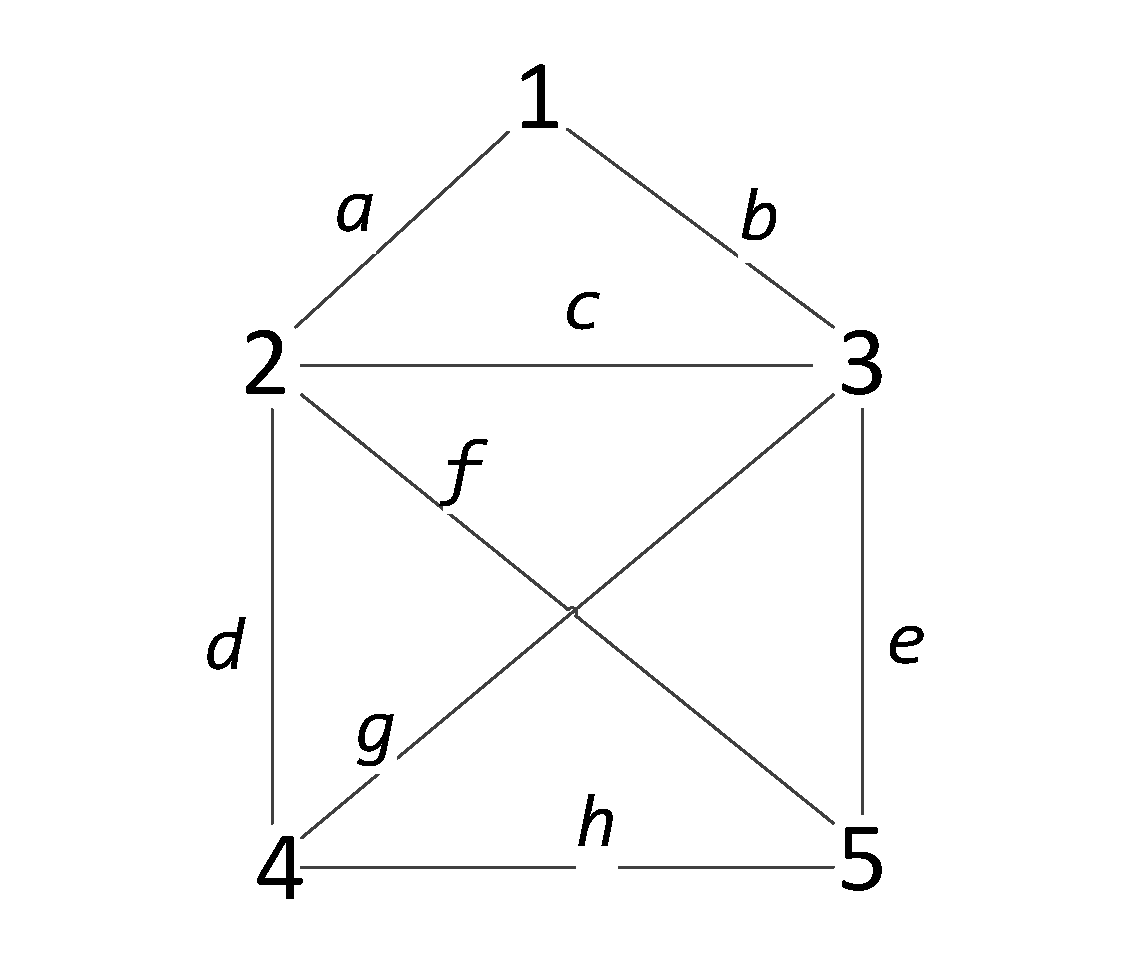
\includegraphics[scale=0.45]{envelope}
	\end{figure}

\end{frame}

\begin{frame}
	
	\frametitle{\insertsection}
	
	\begin{enumerate}
		\setcounter{enumi}{2}
		\item Даны два сосуда объемом 3 и 5 литров. Также имеется источник, из которого можно наполнить сосуды и куда можно вылить лишнюю воду.
		Определить последовательность переливаний, необходимую для получения 4 литров воды в одном из сосудов.
		\item Усовершенствовать решение предыдущей задачи таким образом, чтобы программа принимала на вход начальное состояние:
		целочисленные объемы сосудов V1 и V2, начальное количество воды в каждом сосуде и требуемое количество воды. При этом V1 и V2 взаимно просты.
		По начальному состоянию программа должна определить последовательность переливаний, необходимую для достижения целевого объема.
		Если задача не имеет решения~--- программа должна возвращать \texttt{false}.
	\end{enumerate}
	
\end{frame}


% Формальные грамматики (DCG)

\lecture{Definite clause grammars}{dcg}

\begin{frame}

	\begin{center}
		\Huge Понятие формальных грамматик
	\end{center}

\end{frame}

\section{Понятие формальных грамматик}
\subsection{Интуитивное определение}


\begin{frame}
	
	\frametitle{\insertsection}
	\framesubtitle{\insertsubsection}
	
	Одной из первых и основных областей применения Пролога является компьютерная лингвистика~--- обработка естественных языков
	автоматически. \textbf{Формальная грамматика}~--- это множество правил, которые определяют, какие фразы из заданного алфавита (лексикона)
	являются \textit{синтаксически корректными}. 
	
	Пролог предоставляет средства для описания подобных правил, а, следовательно, для
	задания грамматик, что позволяет проверить любую фразу на корректность относительно заданной грамматики, а также по грамматике 
	сгенерировать все возможные фразы, корректные относительно нее.
	
	Все фразы, синтаксически корректные относительно грамматики, называются \textbf{языком, порождаемым грамматикой}.
	
\end{frame}

\begin{frame}

	\frametitle{\insertsection}
	\framesubtitle{\insertsubsection}
	
	\textbf{Контекстно-свободная} грамматика является частным случаем формальной грамматики.
	
	\begin{table}
		\centering
		\begin{tabular}{ l }
			\rowcolor{LightGray} S \(\rightarrow \) nounPhrase verbPhrase \\
			\rowcolor{LightGray} nounPhrase \(\rightarrow \) article noun \\
			\rowcolor{LightGray} verbPhrase \(\rightarrow \) verbExpr nounPhrase \\
			\rowcolor{LightGray} verbExpr \(\rightarrow \) modalVerb verb prep \\
			\rowcolor{LightGray} article \(\rightarrow \) a \\
			\rowcolor{LightGray} article \(\rightarrow \) the \\
			\rowcolor{LightGray} noun \(\rightarrow \) cat \\
			\rowcolor{LightGray} noun \(\rightarrow \) king \\
			\rowcolor{LightGray} modalVerb \(\rightarrow \) may \\
			\rowcolor{LightGray} verb \(\rightarrow \) look \\
			\rowcolor{LightGray} prep \(\rightarrow \) at
		\end{tabular}
	\end{table}

\end{frame}

\subsection{Дерево разбора}

\begin{frame}
	
	\frametitle{\insertsection}
	\framesubtitle{\insertsubsection}
	
	\begin{itemize}
		\item Данная грамматика содержит 11 правил.
		\item Символ \(\rightarrow \) означает переход в правиле: сущность из левой части правила можно разложить на составляющие таким образом, как указано
		в правой части.
		\item \texttt{S, nounPhrase, verbPhrase, article, noun, verbExpr, modalVerb, verb, prep}~--- нетерминальные символы (нетерминалы).
		\item \textit{a, the, cat, king, may look at}~--- терминальные символы (терминалы). Множество терминалов также называют \textbf{алфавитом} или \textbf{лексиконом}.
	\end{itemize}
	
\end{frame}

\begin{frame}

	\frametitle{\insertsection}
	\framesubtitle{\insertsubsection}
	
	Рассмотрим старую английскую поговорку \textit{A cat may look at a king}.
	
	\begin{figure}
		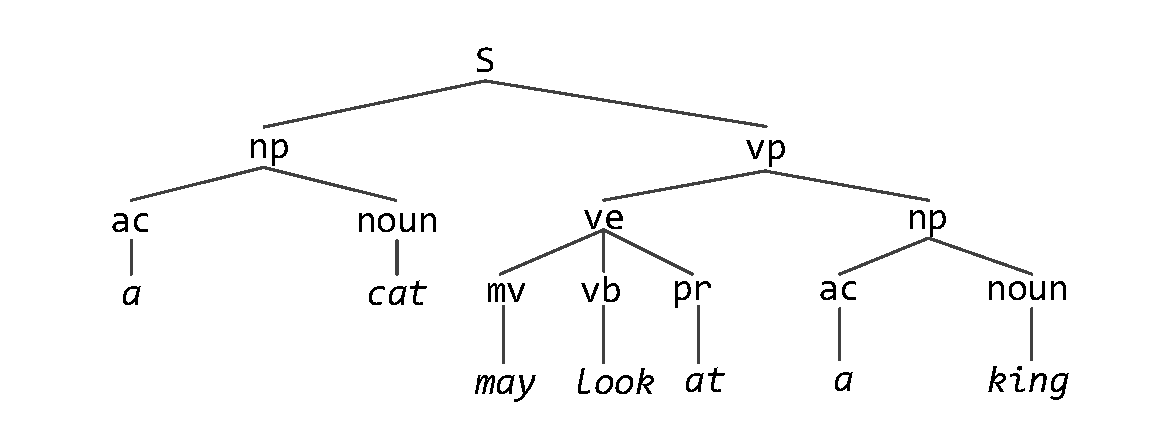
\includegraphics[scale=0.65]{gramtree}
	\end{figure}

\end{frame}


\begin{frame}

	\frametitle{\insertsection}
	\framesubtitle{\insertsubsection}
	
	Дерево разбора (parse tree) содержит информацию о синтаксической корректности и о структуре заданной фразы.
	
	\begin{enumerate}
		\item \textbf{Программа-распознаватель} (recognizer) по заданной строке сообщает, является ли эта строка синтаксически корректной относительно грамматики.
		\item \textbf{Программа-парсер} сообщает, является ли фраза синтаксически корректной и строит parse tree.
	\end{enumerate}

\end{frame}

\subsection{Контекстно-свободные языки}

\begin{frame}

	\frametitle{\insertsection}
	\framesubtitle{\insertsubsection}
	
	\begin{itemize}
		\item \textbf{Контекстно-свободным} называется язык, порождаемый контекстно-свободной грамматикой.
		\item Среди естественных языков контекстно-свободными являются, например, английский, фразцузский и немецкий языки.
		\item Многие языки программирования являются контекстно-свободными языками.
		\item Контекстно-свободные грамматики применяются при разработке компиляторов.
	\end{itemize}
	
\end{frame}

\begin{frame}

	\begin{center}
		\Huge Реализация КСГ на Прологе
	\end{center}

\end{frame}

\section{Реализация КСГ на Прологе}
\subsection{Recognizer}

\begin{frame}

	\frametitle{\insertsection}
	\framesubtitle{\insertsubsection}
	
	Реализуем грамматику, приведенную выше. Сначала опишем правила стандартными средствами Prolog.
	
	\texttt{\begin{itemize}
			\item[] sentense(S) :- nounPhrase(NP), verbPhrase(VP), append(NP,VP,S).
			\item[] nounPhrase(NP) :- article(A), noun(N), append(A,N,NP).
			\item[] verbPhrase(VP) :- verbExpr(VE), nounPhrase(NP), append(VE,NP,VP).
			\item[] verbExpr(VE) :- modalVerb(MV),verb(V),prep(P),append([MV,V,P],VE).
			\item[] article([A]) :- lexicon(''article'', A).
			\item[] noun([N]) :- lexicon(''noun'',N).
			\item[] modalVerb([MV]) :- lexicon(''modal verb'',MV).
			\item[] verb([V]) :- lexicon(''verb'',V).
			\item[] prep([P]) :- lexicon(''prep'',P).
	\end{itemize}}

\end{frame}


\begin{frame}

	\frametitle{\insertsection}
	\framesubtitle{\insertsubsection}
	
	Предикат \texttt{lexicon/2} используется для описания алфавита. Таким образом мы отделяем описание
	доступных нам лексем от описания грамматики. Это удобно.
	
	\texttt{\begin{itemize}
			\item[] lexicon(''article``,''a``).
			\item[] lexicon(''article``,''the``).
			\item[] lexicon(''noun``,''cat``).
			\item[] lexicon(''noun``,''king``).
			\item[] lexicon(''verb``,''look``).
			\item[] lexicon(''modal verb``,''may``).
			\item[] lexicon(''prep``,''at``).
	\end{itemize}}

\end{frame}


\begin{frame}

	\frametitle{\insertsection}
	\framesubtitle{\insertsubsection}
	
	Два предиката для удобства запуска программы. Первый распознает введенную строку, отвечая \texttt{true} или \texttt{false}, а второй генерирует все
	фразы языка, порождаемого грамматикой.
	
	\texttt{\begin{itemize}
			\item[] recognize :- write(''Enter the phrase: ''),\\
			\quad\quad\quad\quad\quad\quad\quad current\_input(In),\\
			\quad\quad\quad\quad\quad\quad\quad read\_string(In, ''\textbackslash n'', ''\textbackslash r\textbackslash t'', \_, Phrase),\\
			\quad\quad\quad\quad\quad\quad\quad split\_string(Phrase,~''~'',~"''',~ListPhrase),\\
			\quad\quad\quad\quad\quad\quad\quad sentense(ListPhrase),!.
			\item[] generate :- sentense(Phrase),\\
			\quad\quad\quad\quad\quad\quad\quad atomics\_to\_string(Phrase,'~',String),\\
			\quad\quad\quad\quad\quad\quad\quad write(String).
	\end{itemize}}

\end{frame}

\begin{frame}

	\frametitle{\insertsection}
	\framesubtitle{\insertsubsection}
	
	Данная программа не будет эффективной.
	
	\begin{itemize}
		\item Она сначала пытается угадать фразу, а затем сравнивает ее с заданной.
		\item Вопрос \texttt{sentense([''a'',''cat'',''may'',''look'',''at'',''a'',''king''])} заставит программу проверять все возможные фразы до тех пор, пока очередная
		не совпадет с нужной.
		\item Причина в том, что в предикаты \texttt{nounPhrase, verbPhrase} и прочие поступают неопределенные переменные, которые требуют означивания.
		\item Это можно исправить, заставив программу сначала разбить фразу на части, а затем проверять эти части на соответствие правилам грамматики.
	\end{itemize}
	
	
\end{frame}


\begin{frame}

	\frametitle{\insertsection}
	\framesubtitle{\insertsubsection}
	
	
	В нашем случае это поможет при распознавании, но сломает генератор языка X\_X
	
	Кроме того, операция \texttt{append} очень дорогая и неэффективная.
	
	\texttt{\begin{itemize}
			\item[] sentense(S) :- append(NP,VP,S), nounPhrase(NP), verbPhrase(VP).
			\item[] nounPhrase(NP) :- append(A,N,NP), article(A), noun(N).
			\item[] verbPhrase(VP) :- append(VE,NP,VP), verbExpr(VE), nounPhrase(NP).
			\item[] verbExpr(VE) :- append([MV,V,P],VE),\\
			\quad\quad\quad\quad\quad\quad\quad\quad modalVerb(MV),\\
			\quad\quad\quad\quad\quad\quad\quad\quad verb(V),\\
			\quad\quad\quad\quad\quad\quad\quad\quad prep(P).
	\end{itemize}}


\end{frame}

\subsection{Разностные списки}


\begin{frame}

	\frametitle{\insertsection}
	\framesubtitle{\insertsubsection}
	
	\textbf{Разностный список} \texttt{L} представляется в виде двух списков \texttt{A} и \texttt{B} таких, что \texttt{L~=~A~\textbackslash~B}.
	Первый список в паре содержит то, что надо оставить, включить в список \texttt{L}, а второй~--- то, что следует отбросить из того, что мы включили.
	Один и тот же список можно представить в виде разностного списка бесконечным числом способов.
	
	\texttt{\begin{itemize}
			\item[] [a, cat, may, look, at, a, king] []
			\item[] [a, cat, may, look, at, a, king, wtf, omg] [wtf, omg]
	\end{itemize}}

\end{frame}


\begin{frame}

	\frametitle{\insertsection}
	\framesubtitle{\insertsubsection}
	
	Так будет выглядеть описание грамматики с разностными списками вместо \texttt{append}.
	
	\texttt{\begin{itemize}
			\item[] sentense(S,D) :- nounPhrase(S,VP), verbPhrase(VP,D).
			\item[] nounPhrase(NP,D) :- article(NP,N), noun(N,D).
			\item[] verbPhrase(VP,D) :- verbExpr(VP,VE), nounPhrase(VE,D).
			\item[] verbExpr(VE,D) :- modalVerb(VE,MV), verb(MV,V), prep(V,D).
			\item[] article([A|D],D) :- lexicon(''article'',A).
			\item[] noun([N|D],D) :- lexicon(''noun'',N).
			\item[] modalVerb([MV|D],D) :- lexicon(''modal verb'',MV).
			\item[] verb([V|D],D) :- lexicon(''verb'',V).
			\item[] prep([P|D],D) :- lexicon(''prep'',P).
	\end{itemize}}

\end{frame}

\subsection{Специальный синтаксис}


\begin{frame}

	\frametitle{\insertsection}
	\framesubtitle{\insertsubsection}
	
	Теперь рассмотрим, какие специальные средства предоставляет Prolog для описания грамматик.
	
	\texttt{\begin{itemize}
			\item[] sentense -{}-\textgreater~nounPhrase, verbPhrase.
			\item[] nounPhrase -{}-\textgreater~article, noun.
			\item[] verbPhrase -{}-\textgreater~verbExpr, nounPhrase.
			\item[] verbExpr -{}-\textgreater~modalVerb, verb, prep.
			\item[] article -{}-\textgreater~[''a''].
			\item[] article -{}-\textgreater~[''the''].
			\item[] noun -{}-\textgreater~[''cat''].
			\item[] noun -{}-\textgreater~[''king''].
			\item[] modalVerb -{}-\textgreater~[''may''].
			\item[] verb -{}-\textgreater~[''look''].
			\item[] prep -{}-\textgreater~[''at''].
	\end{itemize}}

\end{frame}


\begin{frame}

	\begin{center}
		\Huge Рекурсивные правила
	\end{center}

\end{frame}

\section{Рекурсивные правила}
\subsection{Создаем соединительное правило}

\begin{frame}

	\frametitle{\insertsection}
	\framesubtitle{\insertsubsection}
	
	Допустим, мы хотим добавить соединительные правила для генерации бесконечных последовательностей утверждений.
	
	\begin{table}
		\centering
		\begin{tabular}{ l }
			\rowcolor{LightGray} sentense \(\rightarrow \) sentense conjunction sentense \\
			\rowcolor{LightGray} conjunction \(\rightarrow \) and \\
			\rowcolor{LightGray} conjunction \(\rightarrow \) or \\
			\rowcolor{LightGray} conjunction \(\rightarrow \) but \\
		\end{tabular}
	\end{table}
	

\end{frame}


\begin{frame}

	\frametitle{\insertsection}
	\framesubtitle{\insertsubsection}
	
	Нет ничего проще.
	
	\texttt{\begin{itemize}
			\item[] sentense -{}-\textgreater~sentense, conjunction, sentense.
			\item[] conjunction -{}-\textgreater~[''and''].
			\item[] conjunction -{}-\textgreater~[''or''].
			\item[] conjunction -{}-\textgreater~[''but''].
	\end{itemize}}

\end{frame}

\subsection{Что может пойти не так?}

\begin{frame}

	\frametitle{\insertsection}
	\framesubtitle{\insertsubsection}
	
	\begin{itemize}
		\item Если добавить рекурсивное правило в начало, то любой запрос на распознавание фразы приведет к бесконечному циклу и, как следствие, зависанию.
		Это произойдет потому, что в правиле первым стоит рекурсивный вызов. Любой запрос будет натыкаться на первое правило и бесконечно его применять.
		\item Если убрать рекурсивное правило в конец, то синтаксически правильные фразы будут распознаваться, но введение фразы, не являющейся верной в данной
		грамматике, опять-таки приведет к уходу в бесконечный цикл. На этот раз потому, что без возможности применить первое правило мы будем бесконечно пытаться применить второе.
		\item В случае обычной рекурсии такой эффект устраняется перестановкой рекурсивного вызова с первого места дальше. Но в случае грамматик последовательность
		предикатов в теле правила соответствует последовательности слов в синтаксически верных фразах, следовательно мы не можем менять предикаты местами.
	\end{itemize}

\end{frame}

\begin{frame}

	\frametitle{\insertsection}
	\framesubtitle{\insertsubsection}
	
	Так что же делать? \textbf{Вводить дополнительные нетерминалы}.
	
	\texttt{\begin{itemize}
			\item[] plainSentense -{}-\textgreater~nounPhrase, verbPhrase.
			\item[] sentense -{}-\textgreater~plainSentense.
			\item[] sentense -{}-\textgreater~plainSentense, conjunction, sentense.
	\end{itemize}}

\end{frame}

\subsection{Формальные языки}

\begin{frame}

	\frametitle{\insertsection}
	\framesubtitle{\insertsubsection}
	
	Рассмотрим формальный язык \(a^nb^n \). Все слова данного языка состоят из двух последовательностей из равного количества букв \(a\) и \(b\),
	идущих друг за другом. Пустое слово также является словом данного языка.
	
	\uncover<2->{\texttt{\begin{itemize}
			\item[] s --> [].
			\item[] s --> [a],s,[b].
	\end{itemize}}}

\end{frame}

\begin{frame}

	\begin{center}
		\Huge Упражнения
	\end{center}

\end{frame}


\section{Упражнения}

\begin{frame}

	\frametitle{\insertsection}

	\begin{enumerate}
		\item Реализуйте грамматику для языка \(a^nb^n - \{\mathcal{E} \}\).
		\item Реализуйте грамматику для языка \(a^nb^{2m}c^{2m}d^n \).
	\end{enumerate}
	

\end{frame}

\section{Задачи для самостоятельной работы}

\begin{frame}

	\begin{center}
		\Huge \insertsection
	\end{center}

\end{frame}

\begin{frame}

\frametitle{\insertsection}

	Реализовать контекстно-свободную грамматику для проверки корректности S-выражений в языке Clojure.
	Будем рассматривать лишь его подмножество, исключив специфические компоненты.
	
	Основа синтаксиса определяется следующим образом:
	
	\begin{enumerate}
		\item \textbf{Разделитель}. Пробел, табуляция, конец строки, запятая.
		\item \textbf{Атом}.
		\begin{enumerate}
			\item Число. Ограничимся целыми.
			\item Строка. Любая последовательность символов в двойных кавычках.
			\item Идентификатор. Либо последовательность букв, цифр и спецсимволов, начинающаяся с буквы, либо последовательность спецсимволов. Например
			\alert{-\textgreater} является валидным идентификатором. Можно ограничиться спецсимволами \alert{+, -, \textgreater, <, =}.
			\item Ключевые слова. Ключевое слово~--- это идентификатор, предваряемый двоеточием. Например \alert{:Num, :x, :Identifier}.
		\end{enumerate}
		\item \textbf{S-выражение}.
	\end{enumerate}

\end{frame}


\begin{frame}

\frametitle{\insertsection}

	S-выражение рекурсивно строится из атомов, разделителей и скобок.
	
	\begin{itemize}
		\item Любой атом является S-выражением.
		\item Последовательность S-выражений, разделенных разделителями и заключенная в круглые скобки, является S-выражением.
		\textbf{(S1 S2 S3,S4)}.
		\item Последовательность S-выражений, разделенных разделителями и заключенная в квадратные скобки, является S-выражением.
		\textbf{[S1 S2 S3 S4]}.
		\item Последовательность из четного числа S-выражений, разделенных разделителями и заключенная в фигурные скобки, является S-выражением.
		\textbf{\{S1 S2 S3 S4\}}.
	\end{itemize}

\end{frame}


\begin{frame}

\frametitle{\insertsection}

	Программа должна принимать S-выражение, записанное в виде строки, и отвечать \texttt{true} в случае, когда выражение корректно относительно синтаксиса
	языка Clojure, и \texttt{false} в противном случае.
	
	\begin{rexample}
		s\_expression(''(inc 1)``). \\
		s\_expression(''(+ [x y])``). \\
		s\_expression(''((lambda x (nth [(tail x) 0])) (list \textbackslash''Some string\textbackslash``))``).\\
		s\_expression(''\{list (-> A (:List A)),nth (-> (cross (:List A) :Num) (:List A)), tail (-> (:List A)  (:List A))\}``).
	\end{rexample}

\end{frame}



% Операции с файлами и экспорт предикатов

\lecture{Working with files}{files}


\section{Разделение программ и модульность}

\begin{frame}

	\begin{center}
		\Huge \insertsection
	\end{center}

\end{frame}

\subsection{Переиспользование кода}

\begin{frame}

	\frametitle{\insertsection}
	\framesubtitle{\insertsubsection}
	
	\begin{itemize}
		\item[] Чтобы указать интерпретатору о необходимости предварительно прочитать дополнительный код, в начало программы следует добавить список требуемых
		файлов:
		\item[]
		\only<1>{
			\item[] \texttt{:- [source1, source2, \ldots]}
			\item[]
			\item[] Данная инструкция заставит интерпретатор сначала обработать (\textbf{consult}) все файлы из заданного списка, а затем прочитать текущий файл.
		}
		\only<2>{
			\item[] \texttt{ensure\_loaded([source1, source2, \ldots])}
			\item[]
			\item[] Предикат \texttt{ensure\_loaded/1} для каждого указанного файла в списке проверяет, был ли он прочитан ранее, и если да, то изменилось
			ли что-нибудь в нем. Если файл не был прочитан, или с момента последнего чтения был изменен~--- происходит его компиляция. Рекомендуется всегда
			использовать данный предикат вместо более простой предыдущей записи.
		}
	\end{itemize}
	
\end{frame}


\subsection{Модули и экспорт}

\begin{frame}

	\frametitle{\insertsection}
	\framesubtitle{\insertsubsection}
	
	\begin{itemize}
		\item Допустим, у нас имеется 2 файла \texttt{source1.pl} и \texttt{source2.pl}, в которых определены нужные нам предикаты \texttt{func1} и
		\texttt{func2} соответственно. Допустим, также, что в каждом из файлов определен свой предикат \texttt{auxFunc}, от которого зависят
		предикаты \texttt{func1} и \texttt{func2}.
		\item Если мы попытаемся загрузить файлы предыдущим способом, то, скорее всего, мы получим сообщение об ошибке. Либо, что еще хуже, определение
		предиката \texttt{auxFunc} из файла \texttt{source2.pl} затрет предыдущее определение, что может привести к ошибкам в работе предиката \texttt{func1}.
		\item Нашу текущую программу не интересуют зависимости предикатов \texttt{func1} и \texttt{func2}.
	\end{itemize}

\end{frame}


\begin{frame}

	\frametitle{\insertsection}
	\framesubtitle{\insertsubsection}
	
	\begin{itemize}
		\item[] Вместо полной обработки файлов \texttt{source1.pl} и \texttt{source2.pl} мы можем объявить их \textbf{модулями} и экспортировать те предикаты, которые должны быть видны извне.
		\item[]
		\item[] \texttt{:- module(Name, ListOfPredicatesToExport).}
		\item[] \texttt{:- module(mod1, [func1/1]).}
		\item[]
		\item[] Модульность позволяет скрыть определения предикатов, которые нужны только внутри модуля. Предикаты, которые могут быть вызваны снаружи модуля, называются \textit{публичными (public)}, остальные~--- \textit{приватными (private)}.
	\end{itemize}

\end{frame}


\begin{frame}

	\frametitle{\insertsection}
	\framesubtitle{\insertsubsection}
	
	\begin{itemize}
		\item[] Чтобы \textbf{импортировать} модуль, необходимо в начало программы добавить вызов предиката \texttt{use\_module}.
		\item[]
		\only<1>{
			\item[] \texttt{:- use\_module(moduleName).}
			\item[] \texttt{:- use\_module(source1).}
			\item[]
			\item[] Предикат \texttt{use\_module/1} импортирует все public-предикаты из модуля.
		}
		\only<2->{
			\item[] \texttt{:- use\_module(moduleName, ListOfPredicatesToImport).}
			\item[] \texttt{:- use\_module(source1, [func1/1]).}
			\item[]
			\item[] В то время, как \texttt{use\_module/2} позволяет указать список	предикатов, которые необходимо импортировать.
		}
	\end{itemize}

\end{frame}


\subsection{Библиотеки}


\begin{frame}

	\frametitle{\insertsection}
	\framesubtitle{\insertsubsection}
	
	\begin{itemize}
		\item Если при импорте указать, что загружаемый модуль является библиотекой, интерпретатор будет искать его не в текущей директории, а в
		месте хранения библиотек.
		\item \texttt{:- use\_module(library(lib)).}
		\item SWI-Prolog предоставляет множество встроенных предикатов и дополнительных библиотек, в том числе для работы с графическими компонентами.
		\item Другие реализации, например Sicstus, не имеют встроенных предикатов, а весь вспомогательный инструментарий реализован в виде библиотек.
		\item В различных реализациях Пролога один и тот же функционал может быть реализован по-разному, поэтому, если требуется, чтобы программа работала одинаково вне зависимости от интерпретатора, рекомендуется не полагаться на библиотеки и по возможности реализовывать критически важный функционал
		самостоятельно.
	\end{itemize}

\end{frame}


\section{Чтение и запись файлов}

\begin{frame}

	\begin{center}
		\Huge \insertsection
	\end{center}

\end{frame}

\subsection{Открыть файл, закрыть файл}


\begin{frame}

	\frametitle{\insertsection}
	\framesubtitle{\insertsubsection}
	
	\begin{itemize}
		\item[] Прежде, чем можно будет приступить к работе с файлом, его необходимо открыть при помощи предиката \texttt{open/3}.
		\item[]
		\item[] \texttt{open(+FileName,+Mode,-Stream)}
		\item[]
		\item[] Предикат принимает 2 параметра и отдает 1 в качестве результата:
		\begin{itemize}
			\item \texttt{FileName}~--- имя файла. Ничего необычного.
			\item \texttt{Mode}. Режим работы с файлом: \texttt{read, write, append}.
			\item \texttt{Stream}. Уникальный идентификатор потока, присвоенный Прологом.
		\end{itemize}
		\item[] В случае открытия файла в режимах \texttt{write} или \texttt{append} если файла с заданным именем не существует~--- он будет создан.
	\end{itemize}

\end{frame}


\begin{frame}

	\frametitle{\insertsection}
	\framesubtitle{\insertsubsection}
	
	В целом, сеанс связи с файлом выглядит примерно так:
	
	\texttt{\begin{itemize}
		\item[] open(myfile,write,Stream),
		\item[] \ldots
		\item[] do something,
		\item[] \ldots
		\item[] close(Stream),
		\item[] \ldots
	\end{itemize}}

\end{frame}


\subsection{Чтение и запись}

\begin{frame}

	\frametitle{\insertsection}
	\framesubtitle{\insertsubsection}
	
	Для записи в файл используются те же предикаты, что и для вывода в консоль: \texttt{write, writeln, tab, nl}. Только на этот раз
	первым параметром приходится указывать идентификатор потока файла.
	
	\texttt{\begin{itemize}
			\item[] writeFile :- open('out.txt',write,Out), \\ \quad\quad\quad\quad\quad\quad
			write(Out,'Hello,World!'), close(Out).
	\end{itemize}}

	Очевидно, что первым параметром предиката \texttt{open/3} может быть и путь к файлу. Также, может понадобиться предикат \texttt{working\_directory/2},
	если требуется сменить текущую рабочую директорию.

\end{frame}


\begin{frame}

	\frametitle{\insertsection}
	\framesubtitle{\insertsubsection}
	
	Чтение осуществляется предикатом \texttt{read/2}.
	
	\texttt{\begin{itemize}
			\item[] readFile :- open('in.txt',read,In), \\ \quad\quad\quad\quad\quad\quad
			read(In, Input),\\ \quad\quad\quad\quad\quad\quad
			writeln(Input), \\ \quad\quad\quad\quad\quad\quad
			close(Out).
	\end{itemize}}

\end{frame}



% Расширенные возможности грамматик

\lecture{Advanced in DCG}{dcgadv}


\section{Дополнительные аргументы}

\begin{frame}

	\begin{center}
		\Huge \insertsection
	\end{center}

\end{frame}

\subsection{Контекстно-свободные грамматики с параметрами}


\begin{frame}

	\frametitle{\insertsection}
	\framesubtitle{\insertsubsection}
	
	Вспомним грамматику, построенную в прошлый раз.
	
	\begin{table}
		\centering
		\begin{tabular}{ l }
			\rowcolor{LightGray} S \(\rightarrow \) nounPhrase verbPhrase \\
			\rowcolor{LightGray} nounPhrase \(\rightarrow \) article noun \\
			\rowcolor{LightGray} verbPhrase \(\rightarrow \) verbExpr nounPhrase \\
			\rowcolor{LightGray} verbExpr \(\rightarrow \) modalVerb verb prep \\
			\rowcolor{LightGray} article \(\rightarrow \) a \\
			\rowcolor{LightGray} article \(\rightarrow \) the \\
			\rowcolor{LightGray} noun \(\rightarrow \) cat \\
			\rowcolor{LightGray} noun \(\rightarrow \) king \\
			\rowcolor{LightGray} modalVerb \(\rightarrow \) may \\
			\rowcolor{LightGray} verb \(\rightarrow \) look \\
			\rowcolor{LightGray} prep \(\rightarrow \) at
		\end{tabular}
	\end{table}

\end{frame}



\begin{frame}

	\frametitle{\insertsection}
	\framesubtitle{\insertsubsection}
	
	Она порождает фразы следующего вида.
	
	\begin{itemize}
		\item A cat may look at a king
		\item A cat may look at the king
		\item A king may look at a cat
		\item A king may look at the cat
		\item The cat may look at a king
		\item The king may look at a cat
	\end{itemize}

\end{frame}


\begin{frame}

	\frametitle{\insertsection}
	\framesubtitle{\insertsubsection}
	
	OK, допустим, что мы хотим добавить сюда личные местоимения, которые хотим использовать в качестве подлежащего или дополнения.
	
	\begin{itemize}
		\item He may look at her
		\item A cat may look at him
		\item A king may look at her
		\item She may look at a cat
	\end{itemize}

	И тому подобное \ldots
	
\end{frame}


\begin{frame}

	\frametitle{\insertsection}
	\framesubtitle{\insertsubsection}
	
	Добавим немного правил для описания местоимений и правило, указывающее на то, что \texttt{nounPhrase} может состоять не только из
	артикля и имени существительного, но и из местоимения.
	
	\texttt{\begin{itemize}
			\item[] pro -{}-\textgreater ["he"].
			\item[] pro -{}-\textgreater ["him"].
			\item[] pro -{}-\textgreater ["she"].
			\item[] pro -{}-\textgreater ["her"].
			\item[] nounPhrase -{}-\textgreater pro.
	\end{itemize}}

\end{frame}


\begin{frame}

	\frametitle{\insertsection}
	\framesubtitle{\insertsubsection}
	
	Такая грамматика действительно будет распознавать и генерировать фразы, которые мы хотели добавить в язык, но, вместе с тем, и
	другие, синтаксически некорректные с точки зрения английской грамматики.
	
	\begin{itemize}
		\item Him may look at a cat
		\item He may look at she
		\item The king may look at she
		\item The cat may look at she
	\end{itemize}
	
\end{frame}


\begin{frame}

	\frametitle{\insertsection}
	\framesubtitle{\insertsubsection}
	
	\begin{itemize}
		\item DCG~--- это модель, которую мы должны описать самостоятельно, и она не обладает никакими дополнительными знаниями о структуре языка.
		\item В частности, она не знает о правилах построения предложений в английском языке.
		\item В английском \textbf{he} и \textbf{she}~--- это субъектные личные местоимения (\textbf{subjective case}), и они не могут в предложении стоять на
		позиции объектов. Поэтому предложение \textit{A cat may look at she} некорректно.
		\item Аналогично, \textbf{him} и \textbf{her}~--- это объектные местоимения (\textbf{objective case}), соответственно, они не могут стоять на
		суъектной позиции в предложении. Предложение \textit{Him may look at a cat} также некорректное.
	\end{itemize}

\end{frame}


\begin{frame}

	\frametitle{\insertsection}
	\framesubtitle{\insertsubsection}
	
	\begin{table}
		\centering
		\begin{tabular}{| c | c | c | c | c |}
			\hline
			\multirow{2}{*}{\textbf{PERSONS}} & \multicolumn{2}{|c|}{\textbf{SINGULAR}} & \multicolumn{2}{|c|}{\textbf{PLURAL}} \\ \cline{2-5}
			& \textbf{Subjective Case} & \textbf{Objective Case} & \textbf{Subjective Case} & \textbf{Objective Case} \\
			\hline
			\textbf{\(1^{st}\) person} & I & me & we & us \\
			\hline
			\textbf{\(2^{nd}\) person} & you & you & you & you \\
			\hline
			\textbf{\(3^{rd}\) person} & he,she,it & him,her,it & they & them \\
			\hline
		\end{tabular}
	\end{table}

\end{frame}


\begin{frame}

	\frametitle{\insertsection}
	\framesubtitle{\insertsubsection}
	
	Чтобы исправить это, понадобятся дополнительные ограничения, а значит~--- и дополнительные правила в DCG.
	
	\texttt{\begin{table}
			\centering
			\begin{tabular}{l r}
				sentense -{}-\textgreater ~subjNP, verbPhrase. & spr -{}-\textgreater ~~["he"]. \\
				subjNP -{}-\textgreater ~article, noun. & spr -{}-\textgreater ~["she"]. \\
				subjNP -{}-\textgreater ~spr. & opr -{}-\textgreater ~["him"]. \\
				objNP -{}-\textgreater ~article, noun. & opr -{}-\textgreater ~["her"]. \\
				objNP -{}-\textgreater ~opr. & \\
				verbPhrase -{}-\textgreater ~verbExpr, objNP. & \\
			\end{tabular}
	\end{table}}

\end{frame}


\begin{frame}

	\frametitle{\insertsection}
	\framesubtitle{\insertsubsection}
	
	\begin{itemize}
		\item Данное решение работает, но не является эффективным.
		\item Относительно небольшие изменения в лексиконе повлекли значительные изменения в правилах грамматики.
		\item \textbf{He} и \textbf{him} (а также \textbf{she} и \textbf{her}) есть, по сути, одно и то же местоимение, только в разных формах.
		\item Данные формы обладают во многом схожими свойствами.
		\item Полученное решение может быть приемлемым только на очень небольших задачах, т.к. при расширении лексикона и языка мы можем столкнуться с
		необходимостью добавить десятки новых правил.
	\end{itemize}

\end{frame}


\begin{frame}

	\frametitle{\insertsection}
	\framesubtitle{\insertsubsection}
	
	Рассмотрим следующую программу.
	
	\texttt{\begin{table}
			\centering
			\begin{tabular}{l l}
				sentense -{}-\textgreater~ nounPhrase(subj),verbPhrase. & article -{}-\textgreater~ ["a"]. \\
				nounPhrase(\_) -{}-\textgreater~ article, noun. & article -{}-\textgreater~ ["the"]. \\
				nounPhrase(P) -{}-\textgreater~ pro(P). & noun -{}-\textgreater~ ["cat"]. \\
				verbPhrase -{}-\textgreater~ verbExpr, nounPhrase(obj). & noun -{}-\textgreater~ ["king"]. \\
				verbExpr -{}-\textgreater~ modalVerb, verb, prep. & pro(subj) -{}-\textgreater~ ["he"]. \\
				modalVerb -{}-\textgreater~ ["may"]. & pro(subj) -{}-\textgreater~ ["she"]. \\
				verb -{}-\textgreater~ ["look"]. & pro(obj) -{}-\textgreater~ ["him"]. \\
				prep -{}-\textgreater~ ["at"]. & pro(obj) --> ["her"].
			\end{tabular}
	\end{table}}

\end{frame}


\begin{frame}

	\frametitle{\insertsection}
	\framesubtitle{\insertsubsection}
	
	\begin{itemize}
		\item Данное решение \textbf{не содержит новых правил, кроме тех, что нужны для описания новых конструкций языка}.
		\item Можно сказать, что мы ввели новые признаки для описания различных типов предметных выражений (noun phrases).
		\item Дополнительные аргументы в правилах были использованы для того, чтобы показать, какие местоимения могут стоять на позиции субъекта, а какие~--- на позиции объекта.
	\end{itemize}

\end{frame}


\begin{frame}

	\frametitle{\insertsection}
	\framesubtitle{\insertsubsection}
	
	Где располагаются дополнительные аргументы в полной версии правила? Как мы помним, операция \texttt{-{}-\textgreater}~ --- это всего лишь краткая запись
	обычных правил Пролога, где опущены два аргумента, задающие разностные списки.
	
	\texttt{\begin{itemize}
			\item[] sentense -{}-\textgreater~ nounPhrase,verbPhrase.
			\item[] sentense(A,B) :- nounPhrase(A,C),verbPhrase(C,B).
			\item[]
			\item[] sentense -{}-\textgreater~ nounPhrase(subj),verbPhrase.
			\item[] sentense(A,B) :- nounPhrase(subj,A,C),verbPhrase(C,B).
	\end{itemize}}

\end{frame}


\begin{frame}

	\frametitle{\insertsection}
	\framesubtitle{\insertsubsection}
	
	Несмотря на простоту, грамматики с дополнительными аргументами являются мощным иснтрументом для описания сложных синтаксических конструкций.
	Имея представление о том, как задавать DCG с дополнительными параметрами, можно моделировать достаточно сложные языки и решать множество задач.
	Хотя DCG более не используются так широко, как до появления алгоритмов машинного обучения, не стоит недооценивать их эффективность и выразительность.
	В частности, DCG (и регулярные модели) до сих пор используются при разработке компиляторов, морфологических парсеров и лемматизаторов.
	
\end{frame}


\subsection{Построение деревьев грамматического разбора}


\begin{frame}

	\frametitle{\insertsection}
	\framesubtitle{\insertsubsection}
	
	\begin{itemize}
		\item До сих пор наши программы, использующие DCG, могли ответить \textbf{<<да>>} или \textbf{<<нет>>} на вопрос, является ли заданное предложение фразой языка грамматики и сгенерировать все фразы этого языка.
		\item Как правило, такой информации недостаточно, и мы хотим узнать, как именно происходит разбор предложений, т.е. построить дерево разбора (parse tree).
	\end{itemize}

\end{frame}


\begin{frame}

	\frametitle{\insertsection}
	\framesubtitle{\insertsubsection}
	
	\begin{figure}
		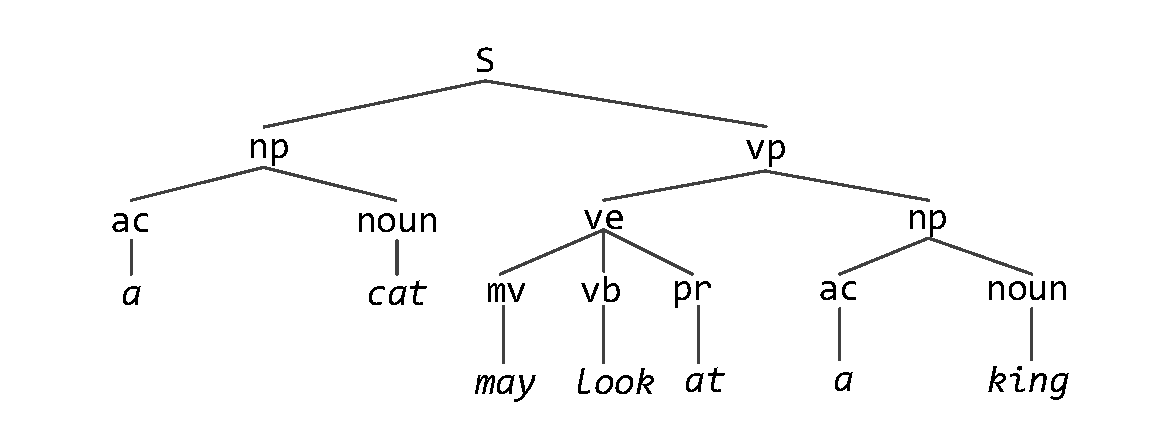
\includegraphics[scale=0.65]{gramtree}
	\end{figure}

\end{frame}


\begin{frame}

	\frametitle{\insertsection}
	\framesubtitle{\insertsubsection}
	
	\texttt{\begin{itemize}
			\item[] sentense(s(NP,VP)) -{}-\textgreater~ nounPhrase(NP), verbPhrase(VP).
			\item[] nounPhrase(np(A,N)) -{}-\textgreater~ article(A), noun(N).
			\item[] verbPhrase(vp(VE,NP)) -{}-\textgreater~ verbExpr(VE), nounPhrase(NP).
			\item[] verbExpr(ve(MV,V,P)) -{}-\textgreater~ modalVerb(MV), verb(V), prep(P).
			\item[] article(art("a")) -{}-\textgreater~ ["a"].
			\item[] article(art("the")) -{}-\textgreater~ ["the"].
			\item[] noun(n("cat")) -{}-\textgreater~ ["cat"].
			\item[] noun(n("king")) -{}-\textgreater~ ["king"].
			\item[] modalVerb(mv("may")) -{}-\textgreater~ ["may"].
			\item[] verb(v("look")) -{}-\textgreater~ ["look"].
			\item[] prep(p("at")) -{}-\textgreater~ ["at"].
	\end{itemize}}

\end{frame}


\begin{frame}

	\frametitle{\insertsection}
	\framesubtitle{\insertsubsection}
	
	Задав в качестве входных данных нашу обычную фразу, получим ответ \texttt{true} и полную структуру разбора.
	
	\begin{itemize}
		\item[] a cat may look at a king
		\item[]
		\item[] s(np(art(''a``), n(''cat``)), vp(ve(mv(''may``), v(''look``), p(''at``)), np(art(''a``), n(''king``)))).
	\end{itemize}

	Очевидно, что такой вид дерева разбора не является обязательным и единственно верным. Для решения задач можно описывать дерево так, как это наиболее удобно для дальнейшей его обработки.

\end{frame}



\section{Дополнительные цели в правилах}

\begin{frame}

	\begin{center}
		\Huge \insertsection
	\end{center}

\end{frame}


\subsection{Реализация контекстно-зависимой грамматики}

\begin{frame}

	\frametitle{\insertsection}
	\framesubtitle{\insertsubsection}
	
	\begin{itemize}
		\item Рассмотрим формальный язык \(a^nb^nc^n-\{\varepsilon \}\). Можно доказать, что данный язык \textbf{не является контекстно-свободным}.
		\item Невозможно описать грамматику, порождающую данный язык, не используя дополнительные параметры. В качестве такого параметра возьмем счетчик букв \(a\), \(b\) и \(c\).
		\item \texttt{s -{}-\textgreater~ ablock(Count),bblock(Count),cblock(Count).}
		\item Блоки из нуля элементов выражаются пустыми строками. Остается определить переход от блока длины \(n+1\) к блоку длины \(n\). Но для этого необходимо задать дополнительные условия.
	\end{itemize}

\end{frame}


\begin{frame}

	\frametitle{\insertsection}
	\framesubtitle{\insertsubsection}
	
	Дополнительные условия записываются в фигурных скобках.
	
	\texttt{\begin{itemize}
			\item[] ablock(0) -{}-\textgreater~ [].
			\item[] ablock(NewCount) -{}-\textgreater~ [a],ablock(Count), \{NewCount is Count + 1\}.
			\item[] bblock(0) -{}-\textgreater~ [].
			\item[] bblock(NewCount) -{}-\textgreater~ [b],bblock(Count), \{NewCount is Count + 1\}.
			\item[] cblock(0) -{}-\textgreater~ [].
			\item[] cblock(NewCount) -{}-\textgreater~ [c],cblock(Count), \{NewCount is Count + 1\}.
	\end{itemize}}

\end{frame}


\begin{frame}

	\frametitle{\insertsection}
	\framesubtitle{\insertsubsection}
	
	Раскрыв <<синтаксический сахар>>, увидим, как выглядят правила Пролога, соответствующие правилам грамматики.
	
	\texttt{\begin{itemize}
			\item[] ablock(NewCount,A,B) :- ’C’(A, a, C), \\ \quad\quad\quad\quad\quad\quad\quad\quad\quad\quad\quad\quad
			 								ablock(Count, C, B), \\ \quad\quad\quad\quad\quad\quad\quad\quad\quad\quad\quad\quad
										 	NewCount is Count + 1.
	\end{itemize}}

	Правило \texttt{'C'(A, a, C)} означает, что мы получим список \texttt{C} из списка \texttt{A}, убрав \texttt{a}.

\end{frame}


\subsection{Разделение правил и лексикона}


\begin{frame}

	\frametitle{\insertsection}
	\framesubtitle{\insertsubsection}
	
	\begin{itemize}
		\item Под разделением правил и лексикона мы будем подразумевать удаление из правил грамматики всех упоминаний конкретных слов. Вместо этого, вся информация о доступных словах записывается в отдельную структуру.
		\item Во-первых, такой подход позволяет более гибко использовать грамматику, так как правила описывают лишь \textit{общие синтаксические шаблоны}, что вполне логично и теоретически позволяет переиспользовать грамматику на разных лексиконах.
		\item Во-вторых, реальные лексиконы могут включать десятки и сотни тысяч слов, для каждого из которых доступно большое количество информации, включая фонологические, морфологические и семантические свойства. Таким образом, мы описываем грамматику, как самостоятельную сущность, и затем используем хранимый отдельно лексикон для эффективного доступа к информации, в частности используя \textbf{First Argument Indexing}.
	\end{itemize}	

\end{frame}	


\section{Выводы}


\begin{frame}

	\frametitle{\insertsection}
	
	\begin{itemize}
		\item Как мы увидели, DCG имеют множество достоинств и позволяют решать задачи, касающиеся анализа как формальных, так и естественных языков.
		\item Решение реальных задач, как правило, требует введения большого числа дополнительных параметров, что делает правила очень громоздкими.
		\item Кроме того, на недостатки самих DCG накладываются и недостатки Пролога, например зацикливание леворекурсивных правил.
		\item При этом, DCG достаточно легко освоить и использовать для описания языков и правил. Язык Prolog предоставляет простые и удобные инструменты для описания DCG. Реализация простой грамматики, подобной той, что была рассмотрена выше, на императивном языке (например C++), потребует гораздо больше времени и строк кода. Это будет проще на функциональном языке (LISP или Haskell), однако их освоение с нуля требует больше времени, чем освоение языка Prolog.
	\end{itemize}

\end{frame}



\section{Задачи для самостоятельной работы}

	\begin{frame}
	
	\begin{center}
		\Huge \insertsection
	\end{center}

\end{frame}


\begin{frame}

	\frametitle{\insertsection}
	
	Усовершенствуйте распознаватель S-выражений таким образом, чтобы превратить его в парсер. В числе прочего, внесите следующие изменения:
	
	\begin{enumerate}
		\item Добавьте в список доступных спецсимволов символ * (звездочка).
		\item Конструкции вида \texttt{()} и \texttt{[]} должны быть синтаксически некорректными, в отличие от \texttt{\{\}}.
		\item Реализовать распознавание \textbf{программ}~--- последовательностей вида \texttt{\{Context\}\_Body}, где в фигурных скобках указан контекст \(\Gamma \), символом \_ (underscore) обозначен любой из доступных разделителей, а
		\texttt{Body}~--- S-выражение.
		\item Пользуясь построенным при помощи парсера деревом синтаксического разбора, реализовать вывод типов S-выражений, являющихся телом программы, правилами расширенного алгоритма Хиндли-Милнера.
	\end{enumerate}

\end{frame}


\subsection{Проверка}

\begin{frame}

	\frametitle{\insertsection}
	\framesubtitle{\insertsubsection}

	Откройте файл \texttt{tasks.clj}. В нем содержатся проверочные задания. Для заданий с 1 по 13 приведены типы соответствующих выражений.
	Задания 14--16 это <<задачи на 5>>.
	
	\begin{enumerate}
		\item Предопределенными типами считаются \texttt{:Int, :Str, :Bool} и \texttt{:List}.
		\item Тестовые программы должны быть прочитаны из файла.
		\item Для каждой тестовой программы в файл с результатами тестов должны быть выведены ее номер, полученный алгоритмом тип, правильный ответ и результат сравнения полученного ответа с правильным.
	\end{enumerate}

\end{frame}


\subsection{Допущения}

\begin{frame}

	\frametitle{\insertsection}
	\framesubtitle{\insertsubsection}
	
	\begin{itemize}
		\item[] Допускается разделение тестовых программ по отдельным файлам.
		\item[]
		\item[] Допускается замена символов переноса строки в тестовых программах на другие разделители (т.е. можно записать программу в одну строчку).
		\item[]
		\item[] Допускается вывод результатов на экран.
	\end{itemize}

\end{frame}


% Дополнительные факты о термах и операторы

\lecture{Advanced in terms}{termadv}


\section{Сравнение термов}

\begin{frame}

	\begin{center}
		\Huge \insertsection
	\end{center}

\end{frame}


\subsection{Унификация и сравнение}


\begin{frame}

	\frametitle{\insertsection}
	\framesubtitle{\insertsubsection}
	
	\begin{itemize}
		\item Язык Prolog, помимо операции унификации \textbf{=} предлагает также предикат~\textbf{==}, реализующий
		сравнение термов.
		\item Ответ на вопрос вида \texttt{term1 == term2.} будет равен \texttt{true} тогда и только тогда, когда термы идентичны друг другу.
		\item Предикат \textbf{==} \textit{не присваивает значения переменным}.
	\end{itemize}

\end{frame}



\begin{frame}

	\frametitle{\insertsection}
	\framesubtitle{\insertsubsection}
	
	Рассмотрим следующие примеры.
	
	\texttt{\begin{itemize}
		\item[] term == term. (true)
		\item[] term1 == term2. (false)
		\item[] term == 'term'. (true)
	\end{itemize}}

\end{frame}


\begin{frame}

	\frametitle{\insertsection}
	\framesubtitle{\insertsubsection}
	
	Теперь добавим переменных.
	
	\texttt{\begin{itemize}
			\item<1->[] X == Y.
			\item<2->[] X == a.
			\item<3->[] X = a, X == a.
			\item<4->[] X = Y, X == Y.
	\end{itemize}}

\end{frame}


\begin{frame}

	\frametitle{\insertsection}
	\framesubtitle{\insertsubsection}
	
	\begin{itemize}
			\item Таким образом, можно сказать, что операции \textbf{=} и \textbf{==} существенно отличаются.
			\item Тем не менее, можно говорить, что \textbf{==} является \textit{более строгим} ограничением, чем \textbf{=}.
			\item Для любых двух термов \texttt{t1} и \texttt{t2}, из того, что выполняется \texttt{t1 == t2}, всегда следует, что \texttt{t1 = t2} также выполняется.
	\end{itemize}

\end{frame}


\subsection{Отрицания операций}

\begin{frame}

	\frametitle{\insertsection}
	\framesubtitle{\insertsubsection}
	
	\begin{itemize}
		\item Операция, обратная сравнению термов \textbf{==}, записывается как \textbf{\textbackslash==}.
		\item Очевидно, что \texttt{t1 \textbackslash== t2} истинно тогда и только тогда, когда \texttt{t1 == t2} ложно.
	\end{itemize}

	\texttt{\begin{itemize}
			\item[] term \textbackslash== term.
			\item[] term1 \textbackslash== term2.
			\item[] term \textbackslash== 'term'.
			\item[] X \textbackslash== a.
			\item[] X \textbackslash== Y.
	\end{itemize}}

\end{frame}


\section{Термы с нестандартной нотацией}

\begin{frame}

	\begin{center}
		\Huge \insertsection
	\end{center}

\end{frame}


\subsection{Арифметические термы}


\begin{frame}

	\frametitle{\insertsection}

	\begin{itemize}
		\item Некоторые термы, которые, на первый взгляд, выглядят по-разному, Prolog интерпретирует как идентичные.
		\item Например, как было показано в примерах выше, термы вида \texttt{term} и \texttt{'term'} идентичны.
		\item В первую очередь, подобные термы нужны для удобства написания кода. Нотации, которые удобны для разбора интерпретатором, обычно не являются удобными для программиста.
		\item Гораздо удобнее писать термы в удобной для себя нотации, чтобы затем интерпретатор разбирал их аналоги, записанные в нотации, удобной для него.
	\end{itemize}

\end{frame}


\begin{frame}

	\frametitle{\insertsection}
	\framesubtitle{\insertsubsection}
	
	Хорошим примером специфических нотаций являются арифметические термы. Как уже было сказано ранее, все арифметические операции \(/, -, *, + \) и другие, являются функторами, а выражения вида \(2 + 3 \)~--- термами.
	
	\texttt{\begin{itemize}
			\item 2+3 == +(2,3).
			\item 2-3 == -(2,3).
			\item 2*3 == *(2,3).
			\item 3*(7+5) == *(3,+(7,5)).
	\end{itemize}}

\end{frame}


\begin{frame}

	\frametitle{\insertsection}
	\framesubtitle{\insertsubsection}
	
	То же касается и арифметических операций сравнения.
	
	\texttt{\begin{itemize}
			\item (2 < 3) == <(2, 3).
			\item (2 =< 3) == =<(2, 3).
			\item (2 =:= 3) == =:=(2, 3).
			\item (2 =\textbackslash= 3) == =\textbackslash=(2, 3).
			\item (2 > 3) == >(2, 3).
			\item (2 >= 3) == >=(2, 3).
	\end{itemize}}

\end{frame}


\begin{frame}

	\frametitle{\insertsection}
	\framesubtitle{\insertsubsection}
	
	Ниже представлены все, известные нам, операции сравнения и их отрицания.
	
	\begin{table}
		\centering
		\begin{tabular}{ c l }
			\multirow{2}{*}{=} & Предикат унификации. Выполняется, если может унифицировать \\ 
			& свои аргументы и фейлится в противном случае. \\
			\textbackslash= & Отрицание унификации. Выполняется в случае провала операции \textbf{=} и наборот. \\
			\multirow{2}{*}{==} & Предикат идентичности. Выполняется, если его аргументы идентичны \\ & и фейлится в противном случае. \\
			\textbackslash== & Отрицание идентичности. \\
			\multirow{2}{*}{=:=} & Предикат арифметического равенства. Выполняется, \\ & если его аргументы числа и равны между собой. \\
			=\textbackslash= & Предикат арифметического неравенства. \\
		\end{tabular}
	\end{table}

\end{frame}


\subsection{Списки как термы}


\begin{frame}

	\frametitle{\insertsection}
	\framesubtitle{\insertsubsection}
	
	\begin{itemize}
		\item Списки также являются хорошим примером user friendly нотации термов.
		\item В привычной записи, список задается путем перечисления его элементов через запятую и заключения их в квадратные скобки.
		\item Пролог задает списки с помощью двух термов: \texttt{[]}, представляющего пустой список, и бинарного функтора \texttt{'.'} для построения непустых списков.
		\item Пустой список это в точности терм \texttt{[]}. Длина такого списка равна 0.
		\item Непустой список имеет вид \texttt{.(term,list)}, где \texttt{term}~--- произвольный терм, а \texttt{list}~--- произвольный список.
	\end{itemize}

\end{frame}


\begin{frame}

	\frametitle{\insertsection}
	\framesubtitle{\insertsubsection}
	
	\texttt{\begin{itemize}
			\item .(a,[]) == [a].
			\item .(f(a,b),[]) == [f(a,b)].
			\item .(a,.(b,[])) == [a,b].
			\item .(a,.(b,.(f(x,y),[]))) == [a, b, f(x,y)].
			\item .(.(.(a,[]),[]),[]) == [[[a]]].
			\item .(a,.(.(b,.(c,[])),.(d.[]))) == [a,[b,c],d].
	\end{itemize}}

\end{frame}


\begin{frame}

	\frametitle{\insertsection}
	\framesubtitle{\insertsubsection}
	
	\begin{figure}
		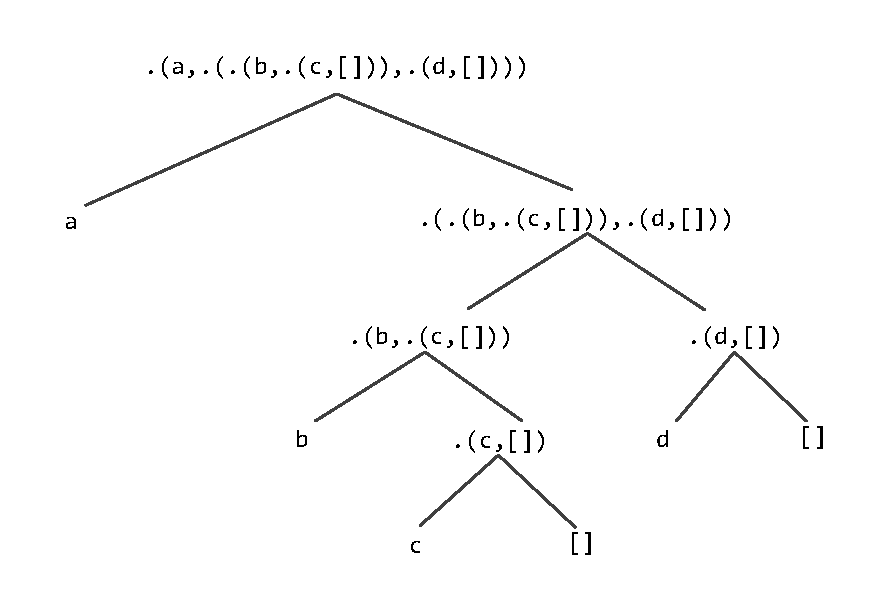
\includegraphics[scale=0.78]{listasterm}
	\end{figure}

\end{frame}


\section{Исследование термов}


\begin{frame}

	\begin{center}
		\Huge \insertsection
	\end{center}

\end{frame}


\subsection{Типы термов}


\begin{frame}

	\frametitle{\insertsection}
	\framesubtitle{\insertsubsection}
	
	\begin{figure}
		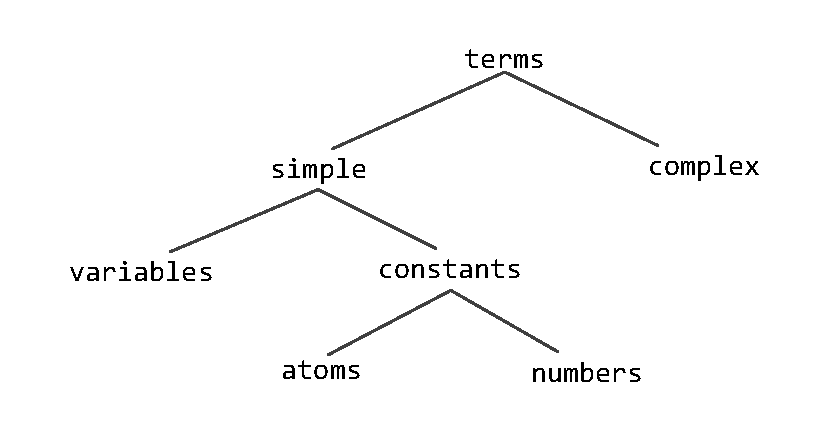
\includegraphics[scale=0.9]{termtypes}
	\end{figure}

\end{frame}


\begin{frame}

	\frametitle{\insertsection}
	\framesubtitle{\insertsubsection}
	
	\begin{table}
		\centering
		\begin{tabular}{ l l }
			\rowcolor{LightGray} \texttt{atom/1} & Проверка, является ли аргумент атомарным \\
			\rowcolor{LightGray} \texttt{integer/1} & Проверка, является ли аргумент целым числом \\
			\rowcolor{LightGray} \texttt{float/1} & Является ли аргумент числом с плавающей запятой \\
			\rowcolor{LightGray} \texttt{number/1} & Является ли аргумент числом (целым или вещественным) \\
			\rowcolor{LightGray} \texttt{atomic/1} & Является ли аргумент константным \\
			\rowcolor{LightGray} \texttt{var/1} & Является ли аргумент неозначенным \\
			\rowcolor{LightGray} \texttt{nonvar/1} & Является ли аргумент означенным
		\end{tabular}
	\end{table}

\end{frame}


\subsection{Структура термов}

\begin{frame}

	\frametitle{\insertsection}
	\framesubtitle{\insertsubsection}
	
	Пусть имеется некоторый терм \texttt{T}, и мы не знаем, как он выглядит, и какие аргументы имеет.
	Какую информацию мы хотели бы знать, чтобы иметь возможность в дальнейшем использовать данный терм?
	
	\uncover<2->{\begin{enumerate}
		\item Каков функтор терма \texttt{T}.
		\item Какова арность терма \texttt{T}.
		\item Каковы аргументы терма \texttt{T}.
	\end{enumerate}}

\end{frame}


\begin{frame}

	\frametitle{\insertsection}
	\framesubtitle{\insertsubsection}
	
	\begin{itemize}
		\item Предикат \texttt{functor/3} отвечает на первые два вопроса.
		\item Принимая на вход составной терм в качестве первого аргумента, он присваивает его функтор и арность своим второму и третьему аргументу соответственно.
	\end{itemize}
	
	Например:
	
	\texttt{\begin{itemize}
		\item[] ?- functor(f(x,y), F, A).
		\item[] F = f
		\item[] A = 2
		\item[] ?- functor(f, F, A).
		\item[] F = f
		\item[] A = 0
	\end{itemize}}

\end{frame}


\begin{frame}

	\frametitle{\insertsection}
	\framesubtitle{\insertsubsection}
	
	При этом, с помощью предиката \texttt{functor/3} мы можем не только находить функторы и арности термов, но и \textbf{конструировать термы с нужными функтором и арностью}.
	
	\texttt{\begin{itemize}
			\item[] functor(T,f,3).
			\item[] T = f(\_21882, \_21884, \_21886).
	\end{itemize}}

	\alert{Обратите внимание, что либо первый, либо второй и третий аргументы должны быть определены.}

\end{frame}


\begin{frame}

	\frametitle{\insertsection}
	\framesubtitle{\insertsubsection}
	
	На третий вопрос о структуре неизвестного терма отвечают два предиката. Один из них~--- это предикат \texttt{arg/3}. Он принимает на вход целое число \(N\), составной терм \texttt{T} и возвращает \(N\)-й аргумент терма \texttt{T}. Также может применяться для присваивания значения \(N\)-му аргументу терма \texttt{T}.
	
	\texttt{\begin{itemize}
		\item[] ?- arg(2, f(x,y), Second).
		\item[] Second = y
		\item[] ?- arg(2, f(x,Y), y).
		\item[] Y = y
		\item[] ?- arg(3, f(x,y), Third).
		\item[] false
	\end{itemize}}

	\alert{Как можно видеть, нумерация аргументов терма начинается с 1.}

\end{frame}


\begin{frame}

	\frametitle{\insertsection}
	\framesubtitle{\insertsubsection}
	
	Вторым предикатом, позволяющим получить доступ к аргументам терма, является \texttt{'=..'/2}. Он принимает составной терм и возвращает список, где первым элементом идет функтор терма, а далее перечислены все его аргументы. Соответственно, задав вопрос \texttt{'=..'(f(x,y), S)}, получим ответ \texttt{S~=~[f,x,y]}. Данный предикат называется \alert{univ} и может использоваться как инфиксный оператор.
	
	\texttt{\begin{itemize}
			\item[] ?- f(x, y, z) =.. Structure.
			\item[] Structure = [f, x, y, z]
			\item[] ?- f(X) =.. F.
			\item[] F = [f, X]
			\item[] ?- T =.. [g, x, y, z].
			\item[] T = g(x, y, z)
	\end{itemize}}

\end{frame}


\section{Операторы}
\subsection{Свойства операторов}

\begin{frame}

	\begin{center}
		\Huge \insertsection
	\end{center}

\end{frame}


\begin{frame}

	\frametitle{\insertsection}
	\framesubtitle{\insertsubsection}

	\alert{Операторы}~--- это функторы бинарных или унарных термов, определенные специальным образом. Существует три типа операторов.
	
	\begin{enumerate}
		\item \textit{Инфиксный оператор} записывается между своими аргументами.
		\item \textit{Префиксный оператор} записывается перед своим аргументом.
		\item \textit{Постфиксный оператор} записывается после своего аргумента.
	\end{enumerate}

\end{frame}


\begin{frame}

	\frametitle{\insertsection}
	\framesubtitle{\insertsubsection}
	
	\begin{itemize}
		\item Каждый оператор имеет \textit{приоритет}.
		\item Например, приоритет операции сложения \(+\) \textbf{выше} приоритета операции умножения \(*\).
		\item Аналогично, приоритет оператора \texttt{is} выше приоритета любой арифметической операции.
		\item Приоритет оператора задается числом от 0 до 1200. Чем больше число, тем выше приоритет.
	\end{itemize}

\end{frame}


\begin{frame}

	\frametitle{\insertsection}
	\framesubtitle{\insertsubsection}
	
	\begin{itemize}
		\item Стандартная нотация выражений в Прологе не имеет неоднозначностей. Например, в выражении \texttt{is(11,+(2,*(3,3)))} всегда понятно, в какой последовательности должны быть выполнены операции.
		\item С другой стороны user friendly нотации могут быть неоднозначны. Выше был пример \texttt{2 =:= 3 == =:=(2,3)}. Операторы \texttt{=:=} и \texttt{==} обладают равными приоритетами, поэтому данное выражение не может быть оценено без постановки скобок.
	\end{itemize}

\end{frame}


\begin{frame}

	\frametitle{\insertsection}
	\framesubtitle{\insertsubsection}
	
	Рассмотрим пример \texttt{X is 1 + 2 + 3}. В данном случае Prolog не выдаст ошибку, а разрешит выражение без постановки скобок.
	
	\texttt{\begin{itemize}
			\item[] ?- 1 + 2 + 3 == +(1, +(2,3)).
			\item[] false
			\item[] ?- 1 + 2 + 3 == +(+(1,2), 3).
			\item[] true
	\end{itemize}}

\end{frame}


\begin{frame}

	\frametitle{\insertsection}
	\framesubtitle{\insertsubsection}
	
	\begin{itemize}
		\item Prolog имеет представление об \textit{ассоциативности} операторов.
		\item Операция сложения левоассоциативна. Это означает, что выражение справа от оператора сложения должно иметь строго меньший приоритет.
		\item Приоритет выражения равен приоритету его оператора или 0.
		\item Операторы \texttt{=:=} и \texttt{==} не имеют ассоциативности.
	\end{itemize}

\end{frame}


\subsection{Описание оператора}

\begin{frame}

	\frametitle{\insertsection}
	\framesubtitle{\insertsubsection}
	
	Определение нового оператора в Prolog выглядит следующим образом:
	
	\texttt{\begin{itemize}
			\item[] :- op(Precedence, Type, Name).
	\end{itemize}}
	
	Соответственно, чтобы задать новый оператор, необходимо знать о нем три вещи:
	
	\begin{enumerate}
		\item Тип (префиксный, инфиксный или постфиксный).
		\item Приоритет.
		\item Ассоциативность.
	\end{enumerate}

\end{frame}


\begin{frame}

	\frametitle{\insertsection}
	\framesubtitle{\insertsubsection}
	
	В описании типа оператора \texttt{f} задает расположение функтора относительно аргументов, которые обозначаются буквами \texttt{x} или \texttt{y}.
	
	\begin{table}
		\centering
		\begin{tabular}{ l l }
			\rowcolor{LightGray} infix & xfx, xfy, yfx \\
			\rowcolor{LightGray} prefix & fx, fy \\
			\rowcolor{LightGray} postfix & xf, yf \\
		\end{tabular}
	\end{table}

	Буквой \texttt{x} обозначается аргумент, приоритет которого должен быть строго меньше приоритета самого оператора, тогда как буквой \texttt{y} обозначается аргумент, приоритет которого может быть меньше либо равным приоритету оператора. Таким образом, оператор типа \texttt{yfx}~--- это инфиксный оператор, обладающий левой ассоциативностью, а оператор \texttt{xfx}~--- инфиксный оператор, не обладающий ассоциативностью.

\end{frame}


\begin{frame}

	\frametitle{\insertsection}
	\framesubtitle{\insertsubsection}
	
	Типы и приоритеты некоторых встроенных операторов.
	
	\texttt{\begin{table}
		\centering
		\begin{tabular}{ l }
			\rowcolor{LightGray} :- op(1200, xfx, [:-, -\textgreater]). \\
			\rowcolor{LightGray} :- op(1200, fx, [:-, ?- ]). \\
			\rowcolor{LightGray} :- op(1200, xfy, [;]). \\
			\rowcolor{LightGray} :- op(1000, xfy, [',']). \\
			\rowcolor{LightGray} :- op(700, xfx, [=, is, =.., ==, \textbackslash==, =:=, =\textbackslash=, <, >, =<, >=]). \\
			\rowcolor{LightGray} :- op(500, yfx, [+, -]). \\
			\rowcolor{LightGray} :- op(500, fx, [+, -]). \\
			\rowcolor{LightGray} :- op(300, xfx, [mod]). \\
			\rowcolor{LightGray} :- op(200, xfy, [\textasciicircum]). \\
		\end{tabular}
	\end{table}}

\end{frame}



% Внутренняя база данных и агрегирование решений

\lecture{Database manipulations and collecting solutions}{dbnag}


\section{Операции с внутренней базой данных}
\subsection{Assert}

\begin{frame}

\begin{center}
	\Huge \insertsection
\end{center}

\end{frame}


\begin{frame}

	\frametitle{\insertsection}
	
	Стандарт языка Prolog предлагает операции для управления динамическими базами знаний, которые могут изменяться в процессе
	исполнения запросов. Основные операции реализуют следующие предикаты:
	
	\texttt{\begin{itemize}
		\item assert/1
		\item asserta/1
		\item assertz/1
		\item retract/1
		\item retractall/1
		\item abolish/1
	\end{itemize}}

\end{frame}


\begin{frame}

	\frametitle{\insertsection}
	\framesubtitle{\insertsubsection}
	
	\begin{itemize}
		\item Допустим, что мы имеем пустую базу знаний, не содержащую ни фактов, ни правил.
		\item В этом случае запрос \texttt{listing.} вернет ответ \texttt{\textbf{true}} и больше ничего.
		\item Выполнив запрос вида \texttt{assert(f(x,y)).} получим ответ \texttt{\textbf{true}}. \textbf{Предикат \texttt{assert} \underline{всегда} завершается успешно.}
		\item Теперь запрос \texttt{listing(f/2).} вернет примерно следующее:
		\texttt{\begin{itemize}
				\item[] :- dynamic f/2.
				\item[] f(x, y).
		\end{itemize}}
	\end{itemize}

\end{frame}



\begin{frame}

	\frametitle{\insertsection}
	\framesubtitle{\insertsubsection}
	
	\begin{itemize}
		\item Во-первых, предикат \texttt{f/2} был объявлен динамическим.
		\item Во-вторых, теперь база знаний содержит факт \texttt{f(x,y).}, соответственно запрос \texttt{f(x,y).} вернет \texttt{true}.
		\item Аналогично можно поступать и с правилами: \texttt{assert((f(X,y) :- (X > 5))).} Здесь мы добавили правило, что \texttt{f(X,y)} выполняется для любых X > 5. Теперь запрос \texttt{f(10,y).} вернет \texttt{true}, а запрос \texttt{f(1,y)}~--- \texttt{false}.
		\item Факт или правило будут добавлены в базу знаний столько раз, сколько раз для них будет вызвана операция вставки.
	\end{itemize}

\end{frame}



\begin{frame}

	\frametitle{\insertsection}
	\framesubtitle{\insertsubsection}
	
	\begin{itemize}
		\item Для более гибкого управления динамической базой знаний используются предикаты \texttt{asserta/1} и \texttt{assertz/1}.
		\item \texttt{asserta/1} добавит выражение в начало динамической базы.
		\item \texttt{assertz/1} добавит выражение в конец.
		\item Предикат \texttt{assert/1} на настоящий момент объявлен устаревшим (deprecated), и его использование не рекомендуется. В SWI Prolog предикат \texttt{assert} работает аналогично \texttt{assertz}.
	\end{itemize}

\end{frame}



\subsection{Retract}


\begin{frame}

	\frametitle{\insertsection}
	\framesubtitle{\insertsubsection}
	
	\begin{itemize}
		\item Для удаления динамических фактов и правил используются предикаты \texttt{retract/1} и \texttt{retractall/1}.
		\item Предикат \texttt{retract/1} удалит первое правило или факт, с которыми сможет унифицировать переданный ему терм.
		\item В случае, если терм нельзя унифицировать с чем-либо в базе знаний, он вернет \texttt{false}.
		\item Предикат \texttt{retractall/1} удалит \textbf{все} вхождения правил или фактов, с которыми сможет унифицировать свой аргумент.
		\item Аргументами предикатов \texttt{retract} и \texttt{retractall} могут выступать как термы, так и правила.
		\item В случае, когда в качестве аргумента передан терм \texttt{T} будут удалены как факты вида \texttt{F.}, так и правила вида \texttt{F :- \ldots} такие, что \texttt{T = F}.
	\end{itemize}

\end{frame}


\subsection{Примеры}


\begin{frame}

	\frametitle{\insertsection}
	\framesubtitle{\insertsubsection}
	
	\only<1>{Добавим в динамическую базу несколько фактов и одно правило.
		
		\texttt{\begin{itemize}
			\item[] assertz(f(x,y)).
			\item[] assertz(f(x,y)).
			\item[] assertz(f(a,b)).
			\item[] assertz((f(X,y) :- g(X,a,b)).
	\end{itemize}}}

	\only<2>{База будет выглядеть примерно так, если задать вопрос \texttt{listing(f/2)}.
		
		\texttt{\begin{itemize}
				\item[] :- dynamic f/2.
				\item[] f(x,y).
				\item[] f(x,y).
				\item[] f(a,b).
				\item[] f(X,y) :- g(X,a,b).
	\end{itemize}}}

	\only<3>{Теперь попробуем удалить одно вхождение факта \texttt{f(x,y)}.
		
		\texttt{\begin{itemize}
				\item[] retract(f(x,y)).
				\item[]
				\item[] f(x,y).
				\item[] f(a,b).
				\item[] f(X,y) :- g(X,a,b).
	\end{itemize}}}
		

	\only<4>{Из оставшегося удалим все факты и правила, такие, что их head унифицируется с термом \texttt{f(X,y)}.
		
		\texttt{\begin{itemize}
				\item[] retractall(f(X,y)).
				\item[]
				\item[] f(a,b).
	\end{itemize}}}

\end{frame}


\begin{frame}

	\frametitle{\insertsection}
	\framesubtitle{\insertsubsection}
	
	Рассмотрим еще один пример~--- вычисление и кеширование таблицы умножения.
	
	\texttt{\begin{itemize}
			\item[] multab(Scale) :- member(X,Scale),\\
			\quad\quad\quad\quad\quad\quad\quad\quad member(Y,Scale),\\
			\quad\quad\quad\quad\quad\quad\quad\quad Prod is X * Y,\\
			\quad\quad\quad\quad\quad\quad\quad\quad assertz(mult(X,Y,Prod)),\\
			\quad\quad\quad\quad\quad\quad\quad\quad fail.
	\end{itemize}}

\end{frame}


\subsection{Abolish}

\begin{frame}

	\frametitle{\insertsection}
	\framesubtitle{\insertsubsection}
	
	\begin{itemize}
		\item Предикаты \texttt{assert(a/z), retract} и \texttt{retractall} работают только с \alert{динамическими фактами и правилами}, т.е. такими, у которых head объявлен динамическим.
		\item Если в базе нет упоминания о предикате \texttt{p}, то при добавлении утверждений с его участием через \texttt{assert} он будет объявлен динамическим.
		\item В противном случае предикат \texttt{p} должен быть объявлен динамическим вручную.
		\item Попытка работать со статическими предикатами при помощи данных операций приведет к ошибке.
		\item Однако, предикат \texttt{abolish/1} дает возможность удалять как статические, так и динамические выражения.
		\item В стандарте \texttt{abolish/1} описан, как предикат, обладающий таким же функционалом, как и \texttt{retractall/1}, однако в SWI Prolog его функционал был расширен, т.к. существование двух предикатов в одинаковым функционалом было признано нецелесообразным.
	\end{itemize}

\end{frame}


\section{Агрегирование решений}
\subsection{Findall}

\begin{frame}

	\begin{center}
		\Huge \insertsection
	\end{center}

\end{frame}


\begin{frame}

	\frametitle{\insertsection}
	
	В случае, когда ответ на запрос предполагает несколько решений, мы можем получить их последовательно поиском с возвратом, либо сначала собрать все возможные решения и получить их в виде списка.
	Следующие три предиката реализуют операции агрегирования решений.
	
	\texttt{\begin{itemize}
			\item findall/3
			\item bagof/3
			\item setof/3
	\end{itemize}}
	
\end{frame}


\begin{frame}

	\frametitle{\insertsection}
	\framesubtitle{\insertsubsection}
	
	Запрос вида
	
	\texttt{\begin{itemize}
			\item[] findall(Buff, Goal, Answers).
			\item[]
	\end{itemize}}

	возвращает список всех возможных значений переменной \texttt{Buff}, удовлетворяющих цели \texttt{Goal}. Чаще всего \texttt{Buff}~--- это просто переменная.
	В случае, когда не удалось найти требуемых значений для \texttt{Buff}, \texttt{findall} возвратит \alert{пустой список}.

\end{frame}


\begin{frame}

	\frametitle{\insertsection}
	\framesubtitle{\insertsubsection}
	
	Например, мы хотим получить все результаты умножения девятки из таблицы умножения.
	
	\texttt{\begin{itemize}
			\item[] findall([X,Y],mult(9,X,Y),Res).
			\item[]
			\item[] Res = [[1,9],[2,18],[3,27],[4,36],[5,45],[6,54],[7,63],[8,72],[9,81]].
	\end{itemize}}
	
\end{frame}


\begin{frame}

	\frametitle{\insertsection}
	\framesubtitle{\insertsubsection}
	
	Параллельно, мы можем задать требуемую структуру элементам результирующего списка.
	
	\texttt{\begin{itemize}
			\item[] findall(nineProds(X,Y),mult(9,X,Y),Res).
			\item[]
			\item[] Res = [nineProds(1,9), nineProds(2,18), nineProds(3,27), nineProds(4,36), nineProds(5,45), nineProds(6,54), nineProds(7,63), nineProds(8,72), nineProds(9,81)].
	\end{itemize}}

\end{frame}


\subsection{Bagof}


\begin{frame}

	\frametitle{\insertsection}
	\framesubtitle{\insertsubsection}
	
	Предикат \texttt{bagof/3} позволяет получить результаты в более упорядоченном виде. Предикат \texttt{findall} возвращает простой мешок решений, в котором собрано все ответы,
	удовлетворяющие заданной цели. При этом, последовательность, в которой расположены эти ответы, зависит только от обхода дерева поиска решений.
	
	Запрос вида
	
	\texttt{\begin{itemize}
			\item[] findall(X,mult(Z,X,\_),Res).
			\item[]
	\end{itemize}}
	
	возвратит что-то похожее на \texttt{[1, 2, 3, 4, 5, 6, 7, 8, 9, 1, 2, 3, 4, 5, 6, 7, 8, 9, 1, 2, 3, 4, 5, 6, 7, 8, 9, 1, 2, 3, 4, 5, 6, 7, 8, 9, 1, 2, 3, 4, 5, 
		6, 7, 8, 9, 1, 2, 3, 4, 5, 6, 7, 8, 9, 1, 2, 3, 4, 5, 6, 7, 8, 9, 1, 2, 3, 4, 5, 6, 7, 8, 9, 1, 2, 3, 4, 5, 6, 7, 8, 9]}
	
	Возможно, это именно то, что нужно, но, очевидно, не всегда такое нас устроит.
	
\end{frame}


\begin{frame}

	\frametitle{\insertsection}
	\framesubtitle{\insertsubsection}
	
	Рассмотрим запрос:
	
	\texttt{\begin{itemize}
			\item[] bagof(X,D\textasciicircum mult(Z,X,D),Res).
			\item[]
	\end{itemize}}
	
	\texttt{bagof} выдаст решения, сгруппированные по Z.
	
	\texttt{\begin{itemize}
			\item[] Z = 1,
			\item[] Res = [1, 2, 3, 4, 5, 6, 7, 8, 9] ;
			\item[] Z = 2,
			\item[] Res = [1, 2, 3, 4, 5, 6, 7, 8, 9] ;
			\item[] Z = 3,
			\item[] Res = [1, 2, 3, 4, 5, 6, 7, 8, 9] ;
			\item[] \ldots
	\end{itemize}}
	
\end{frame}


\subsection{Setof}


\begin{frame}

	\frametitle{\insertsection}
	\framesubtitle{\insertsubsection}
	
	Еще один предикат для агрегирования решений~--- это \texttt{setof/3}. В целом, он работает почти также, как и \texttt{bagof}, за исключением того, что
	\texttt{setof} сортирует агрегированные списки (если может) и удаляет повторяющиеся элементы, т.е. возвращает \textit{упорядоченные множества решений}.

\end{frame}


\begin{frame}

	\frametitle{\insertsection}
	\framesubtitle{\insertsubsection}
	
	Например, запрос
	
	\texttt{\begin{itemize}
			\item[] setof(X,D\textasciicircum Z\textasciicircum mult(Z,X,D),Res).
			\item[]
	\end{itemize}}

	возвратит ответ \texttt{Res = [1, 2, 3, 4, 5, 6, 7, 8, 9]}, в то время, как \texttt{bagof} вернул бы то же самое, что и \texttt{findall}~--- неупорядоченный список всех
	найденных ответов, включая повторы.

\end{frame}



\section{Выводы}

\begin{frame}

	\frametitle{\insertsection}
	
	\begin{itemize}
		\item Динамическая база знаний позволяет кешировать найденные решения для повторного использования и управлять фактами и правилами в процессе выполнения запросов.
		\item При этом, не рекомендуется перегружать программу большим количеством динамических операций, т.к. это сильно затрудняет отладку и читаемость кода.
		\item Операции агрегации решений \texttt{findall, bagof} и \texttt{setof} в совокупности предлагают достаточно возможностей для управления возвращаемыми результатами.
		\item В большинстве случаев будет достаточно \texttt{findall}.
	\end{itemize}

\end{frame}